% Graduation Thesis Template - VNUHCM University of Science, Faculty of Information Technology
% Advanced Program of Computer Science (APCS)
%
% Preferred engine: XeLaTeX (or LuaLaTeX). A pdfLaTeX fallback is provided below,
% so the document also compiles if the build system runs pdflatex.
% Build order: XeLaTeX > Biber > XeLaTeX > XeLaTeX.
% Clean all previously generated build files before rebuilding.

\documentclass[oneside,a4paper,14pt]{extreport}

% Times New Roman per the FIT/HCMUS formatting regulation. TeX Gyre Termes is
% a free, metric-compatible Times clone with full Vietnamese Unicode coverage,
% used via fontspec under XeLaTeX/LuaLaTeX. Under pdfLaTeX the same font is loaded
% through the tgtermes package with T5 (Vietnamese) encoding instead, because
% fontspec raises a fatal error on that engine.
\usepackage{iftex}
\ifPDFTeX
  \usepackage[utf8]{inputenc}
  \usepackage[T5]{fontenc}
  \usepackage{tgtermes}
\else
  \usepackage{fontspec}
  \setmainfont{TeX Gyre Termes}
\fi

% Bibliography
\usepackage[style=ieee, defernumbers=true]{biblatex}
\usepackage{hyperref}
\addbibresource{References/references.bib}

\makeatletter
\def\blx@maxline{77}
\makeatother

% Figures, kept under images/
\usepackage{graphicx}
\graphicspath{ {images/} }

% adjustbox gives \adjustbox{max width=..,max totalheight=..}, which caps a float's
% height as well as its width. Plain \resizebox{\textwidth}{!} only constrains width,
% so tall wide tables/figures overflow the page ("Float too large for page").
\usepackage{adjustbox}

% Source code listings
\usepackage{listings}
\usepackage{color}
\definecolor{codegreen}{rgb}{0,0.6,0}
\definecolor{codegray}{rgb}{0.5,0.5,0.5}
\definecolor{codepurple}{rgb}{0.58,0,0.82}
\definecolor{backcolour}{rgb}{0.95,0.95,0.92}
\lstdefinestyle{mystyle}{
    backgroundcolor=\color{backcolour},
    commentstyle=\color{codegreen},
    keywordstyle=\color{magenta},
    numberstyle=\tiny\color{codegray},
    stringstyle=\color{codepurple},
    basicstyle=\footnotesize,
    breakatwhitespace=false,
    breaklines=true,
    captionpos=b,
    keepspaces=true,
    numbers=left,
    numbersep=5pt,
    showspaces=false,
    showstringspaces=false,
    showtabs=false,
    tabsize=2
}
\lstset{style=mystyle}

% Pseudocode
\usepackage{amsmath}
\usepackage{algorithm}
\usepackage[noend]{algpseudocode}
\makeatletter
\def\BState{\State\hskip-\ALG@thistlm}
\makeatother

% Tables
\usepackage{multirow}
\usepackage{array}
\usepackage{booktabs}
\usepackage{tabularx}

% Math symbols (e.g. \checkmark used in the SLR comparison tables)
\usepackage{amssymb}

% Coloured "Key Takeaways" callout boxes used in the SLR chapter
\usepackage{tcolorbox}

% Keep wide floats from drifting past their section (used by the SLR tables)
\usepackage[section]{placeins}
\newcolumntype{L}[1]{>{\raggedright\let\newline\\\arraybackslash\hspace{0pt}}m{#1}}
\newcolumntype{C}[1]{>{\centering\let\newline\\\arraybackslash\hspace{0pt}}m{#1}}
\newcolumntype{R}[1]{>{\raggedleft\let\newline\\\arraybackslash\hspace{0pt}}m{#1}}

% Chapter heading size
\usepackage{titlesec}
\titleformat{\chapter}[display]
  {\LARGE\bfseries}
  {\chaptertitlename\ \thechapter}{18pt}{\huge}

% 1.5 line spacing (per FIT/HCMUS formatting regulation)
\usepackage{setspace}
\onehalfspacing

\usepackage{indentfirst}

% Margins per official FIT/HCMUS thesis formatting regulation:
% top 3cm, bottom 3.5cm, left 3.5cm, right 2cm
\usepackage[
  top=30mm,
  bottom=35mm,
  left=35mm,
  right=20mm,
  includefoot]{geometry}

% Cover page, and pipeline/flow diagrams in the content chapters
\usepackage{tikz}
\usetikzlibrary{calc,arrows.meta,positioning,shapes.geometric,fit}
\newcommand\HRule{\rule{\textwidth}{1pt}}

% Grouped bar charts (e.g. curated-vs-random dataset comparison, Chapter 5)
\usepackage{pgfplots}
\pgfplotsset{compat=1.18}

% ========================================================================================= %
% Thesis / project metadata - update these to match the signed thesis proposal              %
% ========================================================================================= %
\newcommand{\authorNames}{Phan~Minh~Quang~-~Le~Duc~Phu}
\newcommand{\studentIDs}{22125083~-~22125074}
\newcommand{\thesisTitle}{Evaluating~LLM-based~Android~Malware~Detection}
\newcommand{\advisorNames}{M.Sc.~Trần~Anh~Duy~-~Dr.~Lê~Kim~Hùng}
\newcommand{\program}{Advanced Program of Computer Science}
\newcommand{\faculty}{Faculty of Information Technology}

\begin{document}

\begin{titlepage}

\begin{center}
VNUHCM - UNIVERSITY OF SCIENCE\\
\textbf{\faculty}\\[2cm]


{ \Large \bfseries \authorNames\\[2cm] }

{ \Large \bfseries \MakeUppercase{\thesisTitle} \\[3cm]}

\large GRADUATION THESIS FOR THE BACHELOR OF COMPUTER SCIENCE\\
\large \program\\[2cm]


\begin{tikzpicture}[remember picture, overlay]
  \draw[line width = 2pt] ($(current page.north west) + (2cm,-2cm)$) rectangle ($(current page.south east) + (-1.5cm,2cm)$);
\end{tikzpicture}

\vfill
Ho Chi Minh City, 2026

\end{center}

\pagebreak



\begin{center}

VNUHCM - UNIVERSITY OF SCIENCE\\
\textbf{\faculty}\\[2cm]


{\large \bfseries Phan Minh Quang - 22125083\\}
{\large \bfseries Le Duc Phu - 22125074\\[2cm]}

{ \Large \bfseries \MakeUppercase{\thesisTitle} \\[2cm] }

\large GRADUATION THESIS FOR THE BACHELOR OF COMPUTER SCIENCE\\
\large \program\\[2cm]

\textbf{THESIS SUPERVISORS}\\
\advisorNames

\begin{tikzpicture}[remember picture, overlay]
  \draw[line width = 2pt] ($(current page.north west) + (2cm,-2cm)$) rectangle ($(current page.south east) + (-1.5cm,2cm)$);
\end{tikzpicture}

\vfill
Ho Chi Minh City, 2026

\end{center}
\pagenumbering{gobble}
\end{titlepage}


\cleardoublepage

\pagenumbering{roman}

\phantomsection
\chapter*{Declaration of Authorship}
\label{commitment}
We declare that this thesis is our own work, carried out under the guidance
of \advisorNames.


\addcontentsline{toc}{chapter}{Revision Statement}
\chapter*{Revision Statement}
\label{edit}

\textit{[If the thesis title or content was changed after the defense,
describe the revision here.]}


\addcontentsline{toc}{chapter}{Supervisor's Comments}
\chapter*{Supervisor's Comments}
\label{advisor-comments}

\textit{[Signed comments from the thesis supervisor, provided by the
department office.]}


\addcontentsline{toc}{chapter}{Reviewer's Comments}
\chapter*{Reviewer's Comments}
\label{reviewer-comments}

\textit{[Signed comments from the thesis reviewer, provided by the
department office.]}


\addcontentsline{toc}{chapter}{Acknowledgments}
\chapter*{Acknowledgments}
\label{thanks}

We would like to sincerely thank \ldots


\addcontentsline{toc}{chapter}{Thesis Proposal}
\chapter*{Thesis Proposal}
\label{proposal}

\textit{[Attach the signed thesis proposal (Đề cương khóa luận tốt nghiệp)
submitted to the department office, including the supervisor's signature.]}


% Table of contents, list of figures, list of tables
\addcontentsline{toc}{chapter}{Table of Contents}

\tableofcontents

\cleardoublepage
\addcontentsline{toc}{chapter}{\listfigurename}
\listoffigures

\cleardoublepage
\addcontentsline{toc}{chapter}{\listtablename}
\listoftables

\addcontentsline{toc}{chapter}{List of Abbreviations}
\chapter*{List of Abbreviations}
\label{abbreviations}

\begin{tabular}{ll}
API & Application Programming Interface \\
APK & Android Package (application archive format) \\
APCS & Advanced Program of Computer Science \\
CFG & Control-Flow Graph \\
DL & Deep Learning \\
DNN & Deep Neural Network \\
FNR & False Negative Rate \\
FPR & False Positive Rate \\
GAT & Graph Attention Network \\
LAMD & Name of the framework introduced by Qian et al.~\cite{Qian2025-ua}; the source paper does not spell out an explicit letter-by-letter expansion, but introduces it as ``a practical context-driven framework to enable LLM-based Android malware detection'' \\
LLM & Large Language Model \\
LoRA & Low-Rank Adaptation \\
ML & Machine Learning \\
PICOC & Population, Intervention, Comparison, Outcome, Context \\
PRISMA & Preferred Reporting Items for Systematic Reviews and Meta-Analyses \\
RAG & Retrieval-Augmented Generation \\
SLR & Systematic Literature Review \\
VT & VirusTotal \\
\end{tabular}

\textit{[TODO: keep this list alphabetized and add any further abbreviations
introduced in the chapters, e.g. metric names, tool names.]}


\addcontentsline{toc}{chapter}{Abstract}
\chapter*{Abstract}
\label{summary}

\textit{[Limit: 200-300 words. Use concise, objective academic style,
written as continuous prose (no bullet points). Suggested structure:]}

\begin{enumerate}
    \item \textbf{Context/problem} (1-3 sentences): the background, the
    practical problem or research gap, and why it matters.
    \item \textbf{Objective} (1 sentence): what the thesis specifically
    solves or evaluates.
    \item \textbf{Method} (1-3 sentences): the approach, tools, models, or
    evaluation framework proposed, including notable improvements, and the
    experimental/evaluation method and dataset used, if any.
    \item \textbf{Main results} (1-2 sentences): the key findings, with
    concrete figures where possible (accuracy, speed, dataset size, etc.).
    \item \textbf{Conclusion} (1-2 sentences): the scientific and/or
    practical significance of the results and their applicability.
\end{enumerate}


\clearpage

\pagenumbering{arabic}

% Main content chapters
\chapter{Introduction}
\label{Chapter1}

\section{Motivation and Problem Statement}

\textit{[TODO: Describe the context of Android malware and why detection is
important. Explain the problem this thesis addresses -- evaluating how well
Large Language Models (LLMs) perform at Android malware detection -- and why
existing evaluations are insufficient or incomplete (research gap identified
in the SLR).]}

\section{Research Questions and Objectives}

\textit{[TODO: State the specific research questions the thesis answers, and
the objectives of the evaluation framework, e.g. comparing LLM-based methods
against baselines such as the LAMD framework under consistent datasets and
metrics.]}

\section{Contributions}

\textit{[TODO: Summarize the contributions of this thesis, e.g. (1) a
systematic literature review of LLM-based Android malware detection
approaches, (2) an evaluation framework/methodology for comparing candidate
methods, (3) an empirical comparison of selected methods including one built
on top of the LAMD framework.]}

\section{Thesis Structure}

The remainder of this thesis is organized as follows.
Chapter~\ref{Chapter2} reviews background concepts on Android malware
detection and LLM-based approaches.
Chapter~\ref{Chapter3} presents the first phase of the thesis, a systematic
literature review of LLM-based Android malware detection, and identifies the
research gaps that motivate the evaluation.
Chapter~\ref{Chapter4} presents the proposed evaluation methodology.
Chapter~\ref{Chapter5} reports and discusses the experimental results.
Chapter~\ref{Chapter6} concludes the thesis and outlines future work.


\chapter{Background and Related Work}
\label{Chapter2}

\section{Android Malware Detection}

\textit{[TODO: Introduce Android malware analysis concepts needed to follow
the thesis -- static analysis, dynamic analysis, permissions, API calls,
source/sink taint analysis, etc.]}

\section{The LAMD Framework}

\textit{[TODO: Describe the LAMD framework that one of the evaluated methods
builds on -- its pipeline, inputs/outputs, and why it was chosen as a
baseline/building block.]}

\section{Large Language Models for Security Tasks}

\textit{[TODO: Background on LLMs and how they have been applied to security
and code-analysis tasks in general, before narrowing to malware detection.]}

\section{Related Work}

\textit{[TODO: Summarize the systematic literature review (SLR) findings on
LLM-based Android malware detection approaches. Organize by approach family
(e.g. prompting-based, fine-tuned, agentic/tool-augmented). For each family,
state what problem it solves, its limitations, and how this thesis'
evaluation framework addresses gaps left by prior work.]}


\chapter{Systematic Literature Review}
\label{Chapter3}

This chapter presents the first phase of the thesis: a Systematic Literature
Review (SLR) of LLM-based Android malware detection. Its purpose is to map the
emerging research landscape, consolidate how Large Language Models (LLMs) are
being integrated into detection pipelines, and identify the gaps that the
empirical evaluation in Chapters~\ref{Chapter4} and~\ref{Chapter5} sets out to
address. The review protocol, its four research questions, and the synthesis of
findings are all reported below, together with a threats-to-validity analysis.

\section{Introduction}

The rapid growth of mobile applications has reshaped daily life, with the Android operating system dominating the global market and capturing over 70\% of the total market share~\cite{odea2025android,counterpoint2025smartphones}. This ubiquity has also made Android a primary target for cybercriminals, leading to a continual rise in malware threats that compromise user privacy, financial security, and sensitive data. Modern malware evolves quickly, employing advanced evasion tactics and concealing malicious logic within otherwise legitimate application functions~\cite{mccart2025androidmalware}.

Over the past decade, many learning-based approaches, including conventional machine learning (ML) and deep learning (DL) models, have been developed for Android malware detection~\cite{xu2019droidevolver,kim2019multimodal,cai2021jowmdroid,liu2024unraveling}. Although these models achieve strong detection performance, they face persistent challenges in real-world threat environments. Traditional detectors often suffer from concept drift, where performance degrades when the model is exposed to new or evolving malware variants such as zero-day attacks~\cite{barbero2022transcending}. This problem largely stems from dataset dependencies that introduce bias and limit generalization. In addition, most traditional detection systems operate as ``black boxes'' that offer little in the way of causal, verifiable, or human-readable explanations for their predictions~\cite{pendlebury2019tesseract,Li2024-wl}. Such opacity hinders security analysts from extracting meaningful features, validating outcomes, or translating model insights into actionable defense strategies. Auditing, moreover, often requires systematic, evidence-based reporting rather than a simple summary~\cite{chen2017automated}. In short, many decision-driven solutions rely on statistical correlations within datasets rather than on a genuine understanding of the behavioral semantics underlying complex Android applications~\cite{Li2024-wl}.

The emergence of Large Language Models (LLMs) has introduced a new paradigm for addressing these challenges~\cite{alkaraki2024exploring}. Both general-purpose LLMs (e.g., GPT, Claude, Grok, DeepSeek) and domain-specific code models (e.g., CodeLlama, CodeBERT) show strong capabilities in understanding programming semantics and contextual relationships~\cite{Ruellan2025}. Drawing on vast pre-trained knowledge, LLMs can generalize beyond predefined feature spaces and perform zero-shot inference~\cite{Qian2025-ua}. Their reasoning and generative abilities allow them to analyze complex code structures~\cite{Dong2025}, interpret semantics, and produce natural-language summaries that resemble detailed analyst reports~\cite{He2025-ma}.

Building on these capabilities, recent research has increasingly explored LLMs for fine-grained security tasks that extend beyond simple malware classification~\cite{Zheng2025-no}. LLMs have been used to transform raw static features, such as API calls, permissions, and URLs, into semantically rich functional summaries or descriptive representations of code behavior~\cite{Zhao2024-dw,Shota,Wu2025}. They also support explainability by generating analysis reports that expose the evidence behind a verdict, so that a security analyst can inspect and validate the reasoning rather than accept a bare label. This transparency is what we mean by improving analyst confidence in the model's output~\cite{Li2024-wl,Zhang2025-ot}. LLMs have further been applied to malware auditing and localization, helping to identify malicious functions, establish causal evidence, and construct coherent behavioral narratives~\cite{Zheng2025-no}.

With the rapid and diverse development of these approaches, the field of LLM-based Android malware detection has expanded considerably, producing a wide range of methods, frameworks, and evaluation strategies. This growing body of work remains fragmented, however. Studies adopt different datasets, metrics, and design philosophies, which makes it difficult to compare results or assess collective progress. There is therefore a clear need for a Systematic Literature Review (SLR) that consolidates these methods, synthesizes their findings, and offers a coherent picture of the current research landscape. Such a review can establish a unified perspective, highlight prevailing trends, and identify the gaps and opportunities that will guide the evaluation phase of this thesis.

Accordingly, we conduct an SLR to synthesize emerging methodologies, report their effectiveness as published, and identify promising research directions. Since this area moves quickly and much of its foundational work first appears as preprints, the review deliberately includes grey literature (arXiv preprints) alongside peer-reviewed studies, which gives it the character of a multivocal literature review~\cite{garousi2019mlr}. This review draws on \textbf{6} primary studies that were systematically selected through the screening protocol detailed in Section~\ref{sec:design}. These studies, spanning both benchmarking efforts and novel framework proposals, support the following contributions:

\begin{itemize}
    \item We present a taxonomy of LLM-based techniques for Android malware detection, cataloging the architectural and methodological trends observed across the corpus (RQ1, Section~\ref{sec:rq1}).
    \item We synthesize and report the effectiveness of these approaches relative to conventional baselines as published by the primary studies, covering accuracy, generalization under temporal drift, and computational cost, without attempting a cross-study numerical ranking (RQ2, Section~\ref{sec:rq2}).
    \item We identify critical limitations such as context constraints, computational overhead, and hallucination risks (RQ3, Section~\ref{sec:rq3}).
    \item We outline promising future research directions, emphasizing hybrid architectures, domain-specialized model design, and solutions that enable practical, low-latency deployment (RQ4, Section~\ref{sec:rq4}).
\end{itemize}

The remainder of this chapter is organized as follows. Section~\ref{sec:method} describes the SLR methodology and the guidelines it follows. Section~\ref{sec:design} presents the review protocol, including the research questions, search strategy, eligibility criteria, and study-selection process. Section~\ref{sec:report} reports the synthesis results organized around the four research questions. Section~\ref{sec:threats} discusses threats to validity, Section~\ref{sec:relwork} positions this review against related secondary studies, and Section~\ref{sec:conclusion} summarizes the review.

\section{Methodology}\label{sec:method}

This review was conducted as a Systematic Literature Review (SLR) that charts how Large Language Models (LLMs) are being applied to Android malware detection. The protocol follows established evidence-based software-engineering guidance: the review guidelines of Kitchenham and Charters~\cite{kitchenham2007guidelines}, the snowballing procedure of Wohlin~\cite{wohlin2014guidelines}, and the PRISMA~2020 reporting checklist~\cite{Page2021PRISMA}. Together these keep the search, selection, extraction, and synthesis steps auditable.

This review is not a quantitative meta-analysis. The primary studies use different datasets, labeling policies, and evaluation protocols, so their reported numbers cannot be compared directly. We therefore synthesize the studies methodologically. For each study, we examine how its pipeline is designed, which trade-offs it accepts, and where it performs well or poorly. Section~\ref{sec:report-framing} explains this framing in more detail.

The protocol is organized into three phases:

\begin{enumerate}
    \item \textbf{Planning} -- We articulated the review goal, formulated four research questions, and designed a PICOC-based search strategy. The eligibility criteria were calibrated against pilot retrievals before they were frozen, so that the criteria themselves are explained rather than asserted (Section~\ref{sec:design}).

    \item \textbf{Conducting} -- We executed the search across five digital libraries, deduplicated and screened the records in two stages (title/abstract followed by full-text), and complemented the search with one round of backward and forward snowballing. Records and decisions were managed in Parsif.al~\cite{parsifal} to keep the audit trail consistent across reviewers, and the PRISMA~2020 flow (Figure~\ref{fig:prisma}) captures the per-stage counts.

    \item \textbf{Reporting} -- The retained studies were extracted along a shared data sheet (architecture, LLM role, features, dataset, labeling policy, split strategy, cost, runtime, explainability), then synthesized thematically per research question. We also report the metadata profile of the corpus (Section~\ref{sec:metadata}) and a dedicated threats-to-validity analysis (Section~\ref{sec:threats}).
\end{enumerate}

Two reviewers conducted each stage independently and reconciled disagreements through discussion; ties on borderline papers were resolved by re-reading the full text against the inclusion criteria rather than by majority vote. The protocol, search exports, and screening decisions are stored alongside the manuscript to support reproducibility.

\section{Systematic Literature Review Protocol}\label{sec:design}

\subsection{Research Planning}\label{sec:rqs}

This study adopts an SLR approach to investigate LLM-based techniques and pipelines for Android malware detection. The goals are to characterize how LLMs are integrated into detection workflows, to consolidate the datasets, labeling policies, and evaluation protocols reported in the literature, and to identify research gaps and future directions. The reviewed studies report their results under different conditions, so we do not compare their numbers head to head. The synthesis instead focuses on each study's methodological choices, strengths, and weaknesses, as explained in Section~\ref{sec:report-framing}.

The following research questions operationalize these objectives:

\begin{itemize}
    \item \textbf{RQ1:} What LLM-based techniques have been proposed for Android malware detection?
    \item \textbf{RQ2:} How effective are LLM-based approaches for addressing the problem, and under what evaluation assumptions?
    \item \textbf{RQ3:} What are the challenges and limitations of using LLMs for Android malware detection?
    \item \textbf{RQ4:} What are the potential future improvements in Android malware detection using LLMs, considering the current limitations?
\end{itemize}

\subsection{Search Keywords}\label{sec:keywords}

Search keywords were derived using the PICOC framework (Population, Intervention, Comparison, Outcome, Context)~\cite{petticrew2008systematic} and refined across several pilot searches: synonyms were added when a pilot search missed relevant work, and overly generic terms were dropped when they returned large volumes of unrelated records. Three keyword groups were identified to cover the principal dimensions of the review.

\textit{Group 1 (Population)} captures the target problem domain, encompassing Android malware and related mobile security threats. Synonyms and near-equivalent terms (e.g., ``android malware'', ``mobile malware'', ``APK malware'', ``malicious android'') were included to cover the mobile security landscape and APK-level artifacts.

\textit{Group 2 (Intervention)} enumerates the technologies under examination, namely Large Language Models and their associated methodologies. The group spans general-purpose models, model families, and code-specialized variants to ensure coverage of the full spectrum of LLM techniques applied to malware-related analysis.

\textit{Group 3 (Context)} anchors the search to the deployment environment, specifically security inspection within software and application domains. Studies focused exclusively on privacy rather than security were considered out of scope.

The complete set of terms in each group is listed below:

\begin{itemize}
    \item \textbf{Group 1 (Population):} android malware, mobile malware, APK malware, android threats, mobile threats, malicious android, android security, malicious APK
    \item \textbf{Group 2 (Intervention):} llm, large language model, transformer, prompt, few-shot, gpt, gpt-4, llama, llama2, llama3, llama4, mistral, codellama, starcoder, roberta, codebert, codet5, gemini, claude, qwen
    \item \textbf{Group 3 (Context):} software, security, system, application
\end{itemize}

\subsection{Inclusion and Exclusion Criteria}\label{sec:criteria}

The eligibility criteria are summarized in Table~\ref{tab:inclusion-exclusion} and follow the objectives stated in Section~\ref{sec:rqs}. Criteria I1, I2, E1, and E2 are self-explanatory; we therefore clarify only the criteria whose intent is less obvious.

Criterion E3 excludes opinion and position pieces that report no detection performance, since RQ2 depends on extractable evaluation evidence. Criterion E4 removes papers that mention or use an LLM only outside the detection pipeline, for example for synthetic data generation alone, because such work does not show how LLMs perform detection. Criterion E6 sets the publication cut-off at 2020. We treat the release of GPT-3 in June 2020 as the point at which contemporary LLMs began to show the scale-dependent reasoning, in-context learning, and code-understanding behaviors that this review studies~\cite{brown2020gpt3}. Earlier work mostly relies on small encoder-only models (e.g., early BERT variants) that lack these generative, prompt-driven properties, and the few pre-2020 candidates found during the pilot search confirmed this. Finally, the secondary studies removed under E5 are not discarded outright: they are revisited for comparison in Section~\ref{sec:relwork}.

\begin{table}[htbp]
\centering
\caption{Inclusion and exclusion criteria with rationale}
\label{tab:inclusion-exclusion}
\begin{tabularx}{\columnwidth}{lX}
\toprule
\textbf{ID} & \textbf{Criterion} \\
\midrule
\multicolumn{2}{l}{\textit{Inclusion}} \\
I1 & Studies focused on Android malware detection (platform-specific scope) \\
I2 & Studies using an LLM as a core component of the detection approach \\
\midrule
\multicolumn{2}{l}{\textit{Exclusion}} \\
E1 & Duplicates, posters, and papers without a full-text version \\
E2 & Non-English papers \\
E3 & Papers not reporting detection performance on Android malware \\
E4 & Papers not applying an LLM in the detection methodology \\
E5 & Secondary studies (surveys, reviews, mapping studies) \\
E6 & Papers published prior to 2020 (post-GPT-3 LLM era) \\
\bottomrule
\end{tabularx}
\end{table}

\subsection{Search Process}\label{sec:databases}

We conduct our search from five well-known databases:
\begin{itemize}
    \item ACM Digital Library
    \item IEEE Xplore Digital Library
    \item SpringerLink
    \item Scopus
    \item arXiv
\end{itemize}

These five venues are commonly recommended as starting points for software-engineering SLRs~\cite{kitchenham2007guidelines}. ACM, IEEE, SpringerLink, and Scopus index most peer-reviewed venues in security and software engineering. The fifth source, arXiv, is a grey-literature venue: its manuscripts are published informally and are not peer reviewed. Much of the most recent and most widely cited LLM work in this area exists only as preprints, and omitting them would bias the review toward slower-moving, peer-reviewed work.

The search string was assembled from the three PICOC-derived keyword groups described in Section~\ref{sec:keywords}, combining them as follows:

\begin{quote}
(G1-1 OR G1-2 OR $\ldots$) AND (G2-1 OR G2-2 OR $\ldots$) AND (G3-1 OR G3-2 OR $\ldots$),
\end{quote}

\noindent where G$x$-$y$ denotes the $y$-th term of Group $x$.

Queries were executed across the five databases listed above on 1~November 2025. Results were ranked by relevance, with a cap of 400 studies per database applied to bound the screening workload. For arXiv, the threshold was reduced to 200 articles to account for the elevated proportion of pre-publication manuscripts. All metadata were exported and imported into Parsif.al~\cite{parsifal} to support structured management and screening. The raw database yields were: ACM Digital Library (346), arXiv (210, capped from a larger pool), IEEE Xplore (77), Scopus (400, capped), and SpringerLink (400, capped), for a total of 1{,}433 records before deduplication.

\subsection{Study Selection}\label{sec:selection}
Article selection followed a two-stage screening procedure anchored to the eligibility criteria in Section~\ref{sec:criteria}. A study was retained only if it satisfied all inclusion criteria (I1 and I2) and triggered none of the exclusion criteria (E1--E6). Meeting a single inclusion criterion was not sufficient, whereas matching any one exclusion criterion was enough to reject a study.

In the first stage, we screened each record on its title, abstract, keywords, and conclusion, examined in that order. The exclusion criteria were applied first: a record that clearly matched any exclusion criterion was removed immediately, while records that appeared relevant or remained ambiguous were carried forward. In the second stage, the two reviewers independently read the full text of each surviving candidate and confirmed that all inclusion criteria were met and no exclusion criterion applied before agreeing on a final decision. Applying the exclusion criteria first kept the costly full-text reading focused on records that were already plausibly in scope. After both stages, \textbf{5} studies were retained.

To complement the database search and improve overall coverage, backward and forward snowballing were carried out in accordance with Wohlin's guidelines~\cite{wohlin2014guidelines}. Backward snowballing involved a systematic review of the reference sections of all included studies, targeting relevant works that the keyword-based search may have missed. Forward snowballing involved querying Google Scholar to retrieve all articles that had cited papers in the current pool. Candidate studies identified through both directions were subjected to the same inclusion and exclusion criteria applied during primary screening. This process yielded \textbf{1} additional study, bringing the final set to \textbf{6} included papers. The final pool was completed on December~12, 2025, and the list of included studies is presented in Table~\ref{tab:selected-papers}.

\begin{figure}[htbp]
    \centering
    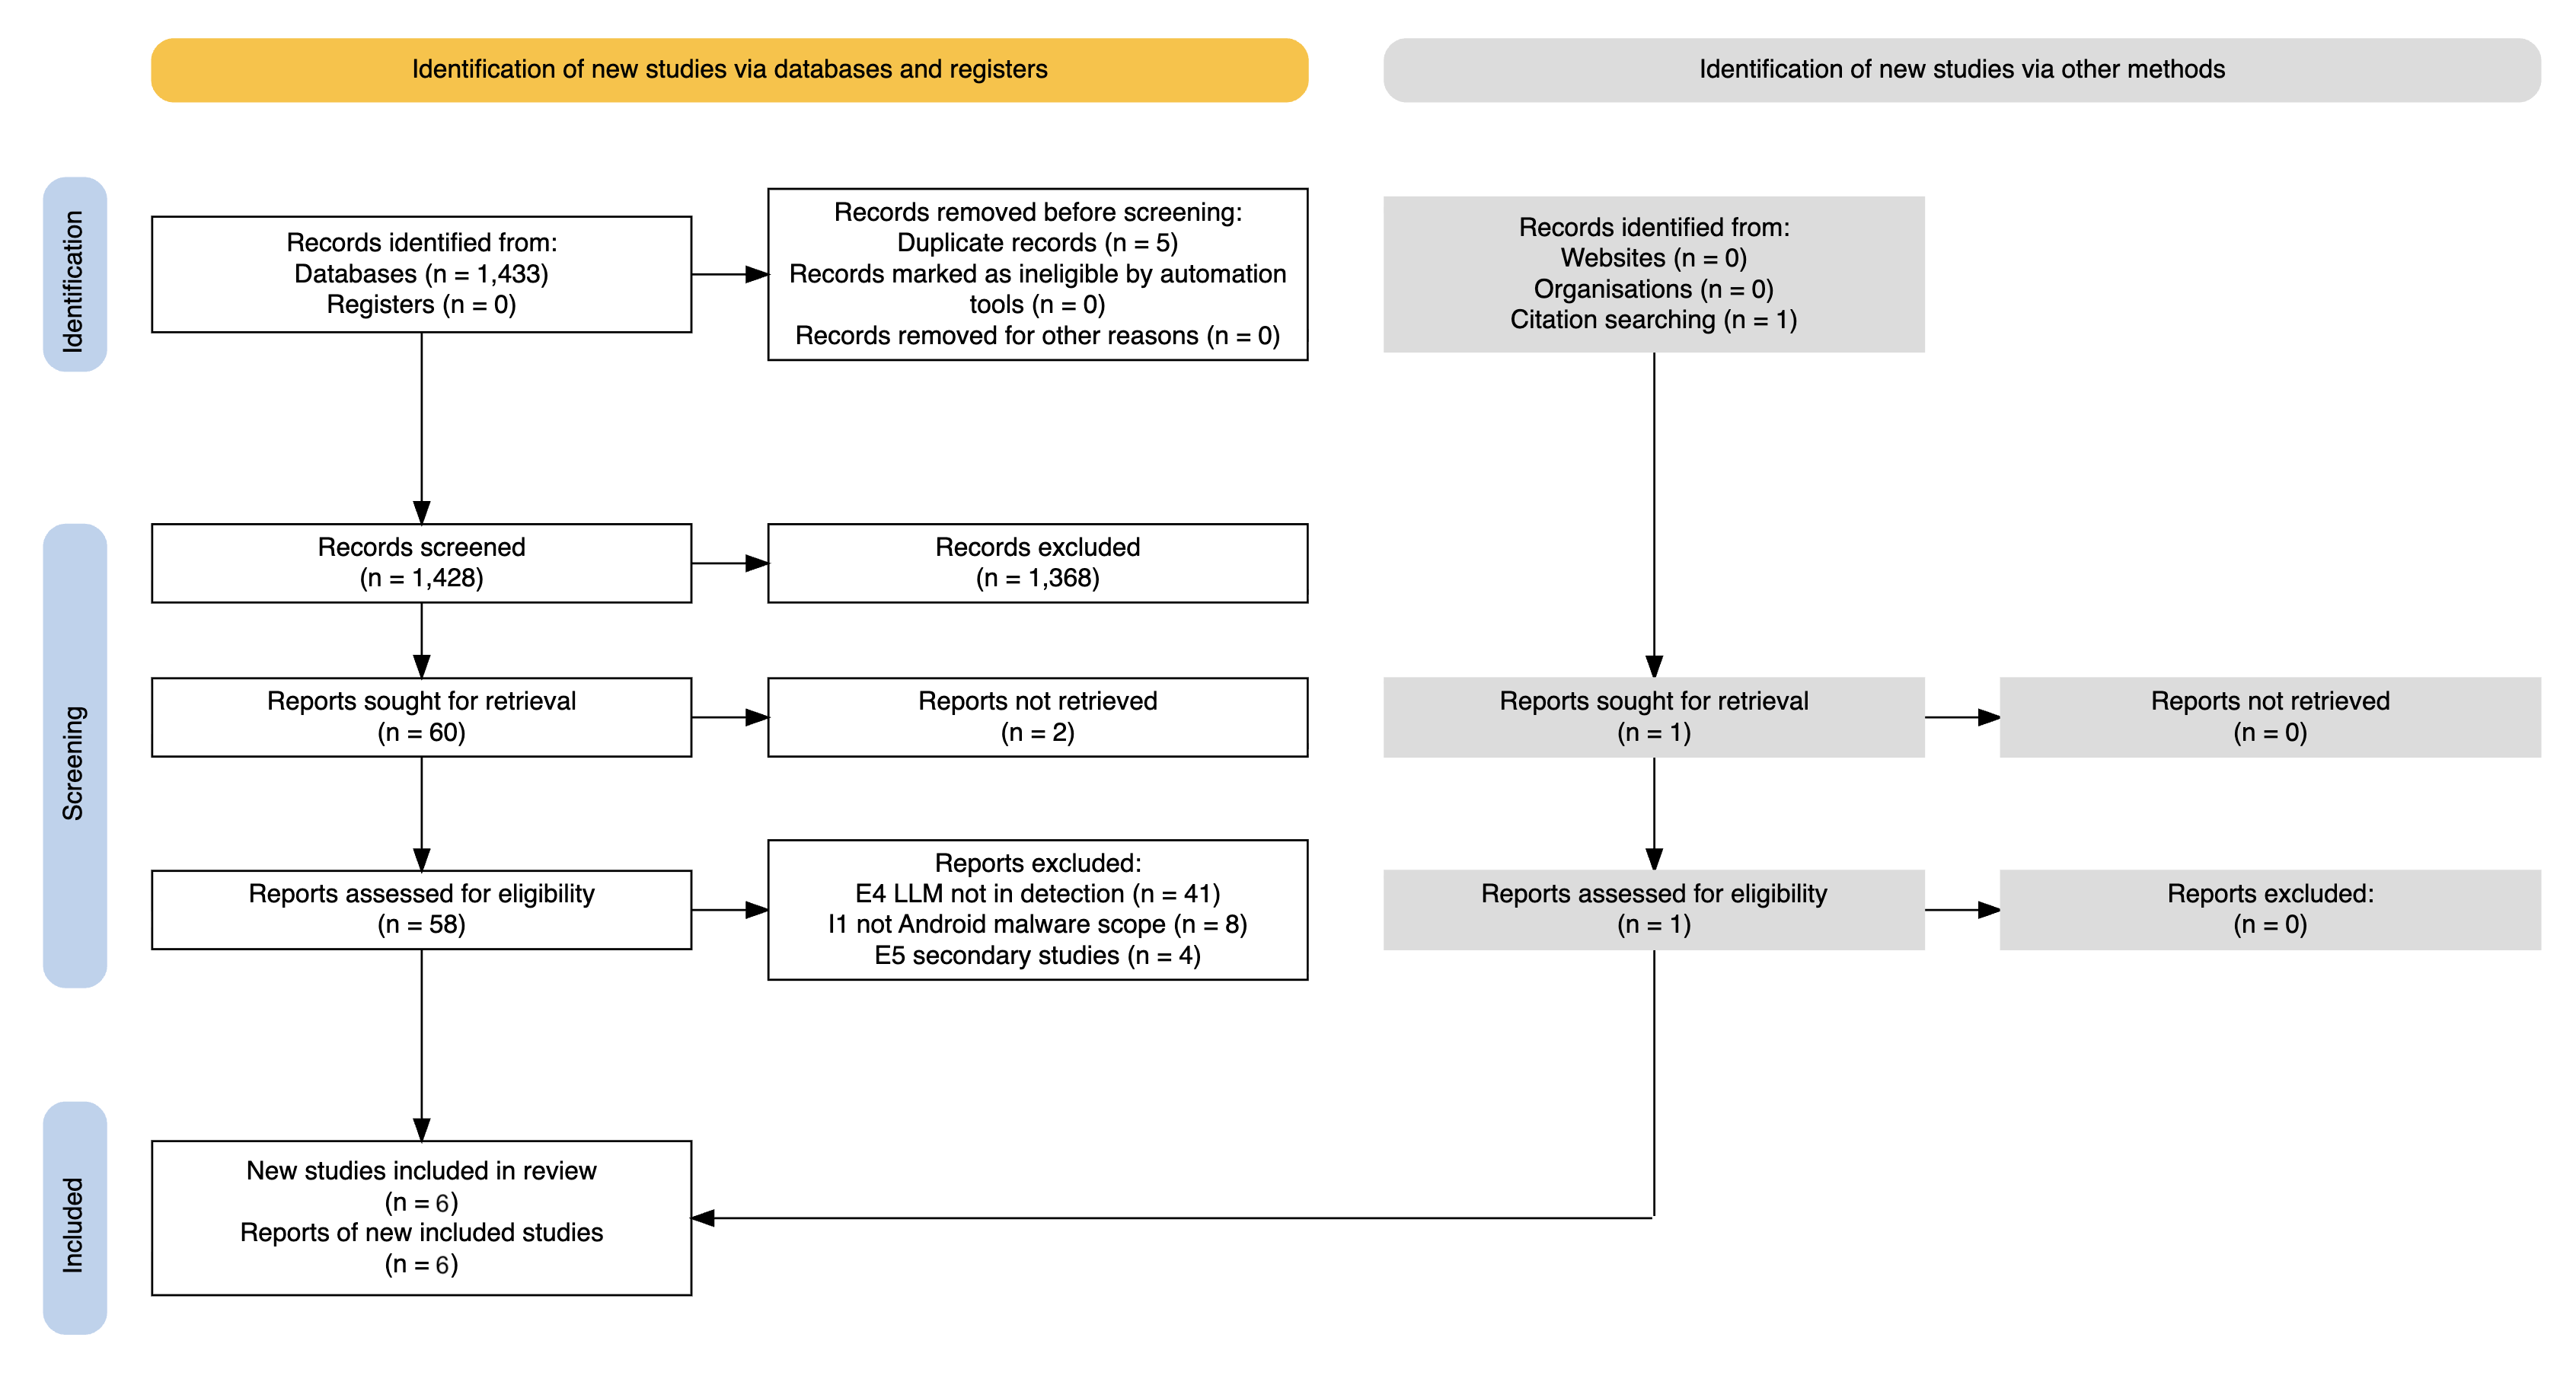
\includegraphics[width=0.95\textwidth]{prisma.png}
    \caption{PRISMA diagram of the selection process.}
    \label{fig:prisma}
\end{figure}

\begin{table}[htbp]
\centering
\caption{List of selected studies}
\label{tab:selected-papers}
\begin{tabularx}{\textwidth}{Xll}
\toprule
\textbf{Title} & \textbf{Author(s)} & \textbf{Year} \\
\midrule
A structural-semantic approach integrating graph-based and LLM representation~\cite{Khan2024-hy}         & Khan \& Kwon  & 2024 \\
AppPoet: LLM-based Android malware detection via multi-view prompt engineering~\cite{Zhao2024-dw}        & Zhao et al.   & 2024 \\
Enhancing Android malware detection with Retrieval-Augmented Generation~\cite{S2025-kj}                  & Saraga et al. & 2025 \\
LAMD: Context-driven Android malware detection and classification with LLMs~\cite{Qian2025-ua}           & Qian et al.   & 2025 \\
LLM-MalDetect: A large language model-based method for Android malware detection~\cite{Feng2025-ry}      & Feng et al.   & 2025 \\
TraceRAG: A LLM-based framework for explainable Android malware detection~\cite{Zhang2025-ot}            & Zhang et al.  & 2025 \\
\bottomrule
\end{tabularx}
\end{table}

\section{Reporting Results}\label{sec:report}

\subsection{Overview of Selected Articles}

The six studies retained after screening were all published in 2024--2025. This narrow window reflects how recently LLMs have been adopted for Android malware detection and indicates that the field is still in a formative stage. Despite the short timespan, the studies differ considerably in how they use LLMs, ranging from retrieval-augmented reasoning over decompiled source code to fine-tuning compact open-source models on structured feature sets, and from multi-view prompt engineering to hybrid graph-and-embedding designs. The detailed findings behind these differences are presented under the four research questions defined in Section~\ref{sec:design}; here we set out only the framing of the synthesis and the publication-level profile of the corpus.

To complement the per-question synthesis, we also summarize the publication-level characteristics of the six retained studies (Table~\ref{tab:metadata}).\label{sec:metadata} Three observations follow from Table~\ref{tab:metadata}. First, the corpus is heavily skewed toward 2025 and toward arXiv preprints; this reflects the recency of LLM adoption and means that several findings have not yet completed peer review -- a point we revisit in Section~\ref{sec:threats}. Second, although the corpus is small, it is geographically distributed and is not dominated by a single lab: the Cavallaro group at King's College London is the most prolific cluster (LAMD and two related benchmarking studies that we cite as context), but four of the six retained primary studies come from independent groups. Third, half of the corpus releases code or prompts publicly, which constrains how reliably the remaining studies can be replicated and is a recurring driver of the comparability concerns in Section~\ref{sec:threats}.

\begin{table}[htbp]
\centering
\caption{Metadata profile of the six retained studies}
\label{tab:metadata}
\footnotesize
\begin{tabularx}{\columnwidth}{lX}
\toprule
Attribute & Value \\
\midrule
Publication years & 2024 (2), 2025 (4) \\
Venue types & 4 preprints (arXiv), 1 journal (IEEE Access), 1 book chapter (IFIP/Springer) \\
Top author affiliation regions & UK/EU (Cavallaro group: LAMD), Asia (Zhao, Feng, Khan, Zhang), South-Asia/EU collab.\ (Saraga et al.) \\
Most frequent author cluster & Cavallaro group at King's College London (LAMD)~\cite{Qian2025-ua} and benchmarking work~\cite{He2025-ma,Zheng2025-no} \\
Recurring co-authors & Qian, Zheng, He, Cavallaro appear in LAMD, benchmarking, and behavior-auditing papers \\
Geographic spread & China (3), South-Korea (1), Italy/India (1), UK (1) \\
Open-source artifact released? & 3/6 (LAMD, AppPoet, AgenticRAG); not released by TraceRAG, LLM-MalDetect, Structural-Semantic \\
LLM backbone family & GPT-4 / GPT-4o-mini / o3-mini (3), Gemini Flash (1), Mistral-7B + LoRA (1), CodeBERT (1) \\
\bottomrule
\end{tabularx}
\end{table}

\renewcommand{\arraystretch}{1.25}
\setlength{\tabcolsep}{6pt}

\section{RQ1: What LLM-based techniques have been proposed
for Android malware detection?}\label{sec:rq1}

\subsection{Background: Android Malware and Its Detection}

Android malware refers to applications that carry out harmful actions on a device, such as stealing personal data, intercepting credentials, sending premium-rate messages, displaying fraudulent payment screens, or covertly tracking the user. Such applications reach devices through app marketplaces or sideloading and frequently disguise their malicious logic inside otherwise functional apps. An Android application is distributed as an APK package that contains a manifest (declaring permissions and components), compiled DEX bytecode, resources, and native libraries; these artifacts are the raw material that any detector inspects.

Detection techniques are conventionally grouped into static, dynamic, and hybrid analysis. Static analysis inspects the APK without executing it, extracting features such as requested permissions, API calls, opcode sequences, and call graphs. Dynamic analysis runs the app in a sandbox and observes behavior such as system calls and network traffic, while hybrid analysis combines both. Over the past decade, machine-learning and deep-learning classifiers built on these features have become the dominant approach. The studies reviewed in this section build on the static branch of this tradition but replace, or augment, the conventional classifier with an LLM. The remainder of this subsection groups the reviewed work by the role the LLM plays in the pipeline.

\subsection{Overview of Strategies}

Based on the studies reviewed, LLM-based Android malware detection approaches generally follow three strategies, distinguished by the role the LLM plays:

\begin{itemize}
    \item \textit{Retrieval-Augmented Generation} -- the LLM filters and retrieves the relevant parts of an application, for example by removing unreachable paths, summarizing methods for indexing, or re-ranking retrieved snippets to reduce noise before analysis.
    \item \textit{Semantic Representation} -- the LLM turns raw features into structured abstractions, such as per-feature notes, hierarchical summaries from functions to packages, or embeddings attached to graph nodes, so that later stages can reason over a cleaner view.
    \item \textit{Fine-tuning and Direct Classification} -- the model is adapted to the detection task through training, either by fine-tuning an LLM on unified textual inputs (e.g., LoRA) or by training a dedicated classifier on LLM-derived representations, so that it emits the verdict directly.
\end{itemize}

Figure~\ref{fig:group1_arch} shows how the three strategies share a common context-construction stage, which decompiles the APK and prepares embeddings and code descriptions, and then diverge in how the LLM is used to reach a verdict. These strategies also overlap in practice: many systems combine LLM-driven context curation, semantic transformation, and a trained classifier. The following subsections describe representative approaches within each strategy.

\begin{figure}[htbp]
    \centering
    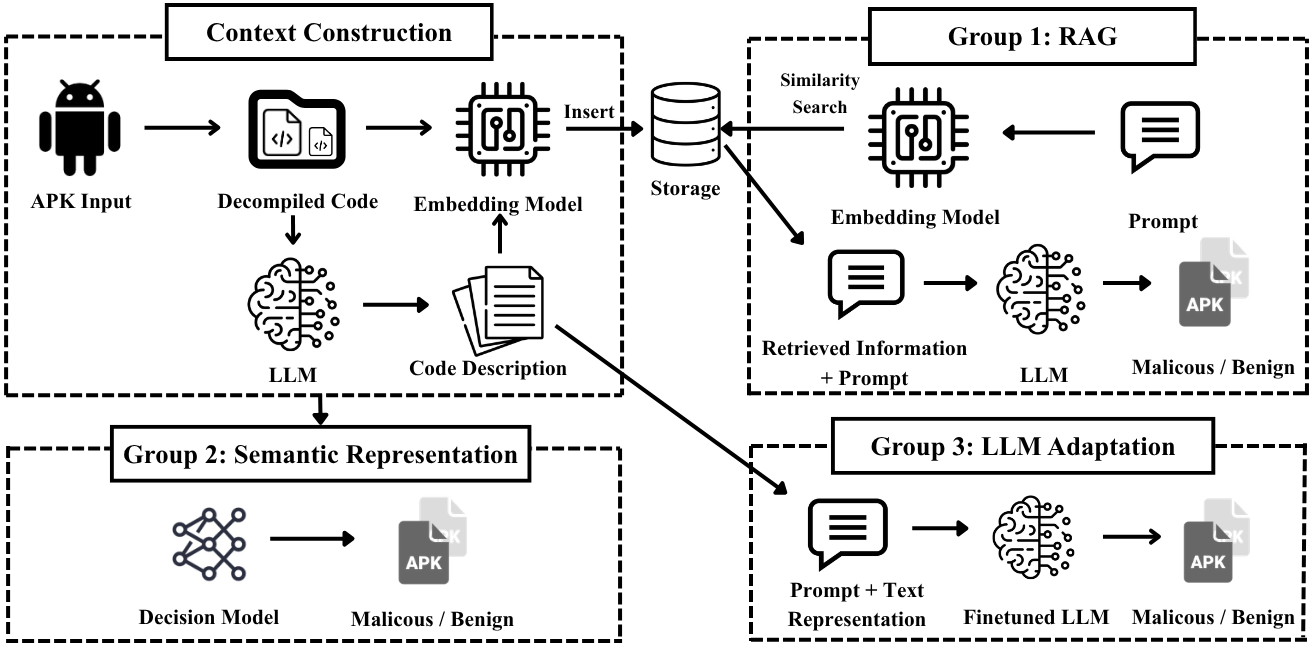
\includegraphics[width=\textwidth]{rq1_diagram_v5.png}
    \caption{General architecture of the reviewed LLM-based Android malware detection pipelines.}
    \label{fig:group1_arch}
\end{figure}

\subsection{Retrieval-Augmented Generation}

Approaches in this category adopt Retrieval-Augmented Generation (RAG)~\cite{Lewis2020-rag}, which augments model inference by retrieving relevant external context at query time instead of relying only on parametric knowledge. For Android malware detection, this means selecting, filtering, and organizing the relevant code and features before reasoning or classification. The shared aim is to reduce the complexity of an application, which often contains large amounts of irrelevant or obfuscated code, by pruning dead paths, summarizing methods, or re-ranking retrieved snippets. Directing the LLM's attention to the most informative parts of the app improves both efficiency and interpretability. The resulting pipelines pair RAG with static program analysis and keep context preparation separate from decision-making, so later stages operate on cleaner, more focused representations.

TraceRAG~\cite{Zhang2025-ot} and AgenticRAG~\cite{S2025-kj} are two examples that emphasize retrieval and explainable analysis. TraceRAG organizes its pipeline as a set of named LLM-driven modules. An \emph{LLM-Describer} produces method-level summaries that are indexed into a vector store, and an \emph{LLM-Cleanser} prunes dead or unreachable code to reduce obfuscation noise. Retrieval runs in two steps: top-$k$ similarity search, followed by an \emph{LLM Relevance-Reviewer} that keeps only the snippets aligned with the suspected behavior. An \emph{LLM-Analyzer} then reasons over the retrieved code in a depth-first, multi-turn manner, asking follow-up questions to reconstruct execution chains that may involve dynamic loading, reflection, or callbacks. Finally, an \emph{LLM-Organizer} compiles a report that cites concrete code locations and call chains, yielding traceable findings.

AgenticRAG takes a feature-driven route. It starts from static features such as permissions, intents, receivers, and services, and has an LLM write a functional description of each. These descriptions are retrieved with an ensemble retriever that combines FAISS~\cite{faiss_lib} and BM25~\cite{Robertson2009} through Reciprocal Rank Fusion, using exact matching first and then fuzzy (Levenshtein) matching to tolerate partial or misspelled names. The retrieved descriptions are classified by domain-specific transformers, namely CySecBERT~\cite{Bayer2024} and SecBERT~\cite{Huang2024}, while a lightweight cache supports modular workflows and a Gemini Fusion model serves as a baseline. Both systems stress interpretability and coverage, but their quality depends on retrieval choices (indexing granularity and prompt alignment) and on the cost of multi-turn reasoning.

\subsection{Semantic Representation}
Approaches in this category transform raw code and features into structured, high-level representations that are easier for an LLM to reason over. The aim is to capture the semantic essence of an application, such as function behaviors, API usage patterns, or hierarchical program structure, while discarding irrelevant low-level detail. Per-feature notes, hierarchical summaries, or node embeddings let the LLM reason over complex apps in a scalable, systematic way. Such representations also help maintain context across large codebases and support modular, multi-level analysis.

AppPoet~\cite{Zhao2024-dw} pairs prompted semantic views with a lightweight classifier. Static features are organized into three views, Permission, API, and URL/uses-feature, so the LLM reasons within coherent contexts. For each view, the LLM uses chain-of-thought prompting to generate per-feature function notes and a view-level summary. These texts are embedded (e.g., with text-embedding-ada-002), concatenated, and passed to a compact MLP that produces the binary verdict, and the LLM also drafts a human-readable diagnostic report. The design is modular and data-efficient because it decouples expensive LLM reasoning from the final decision. Its performance, however, is sensitive to how the views are defined and to the prompt and embedding choices, and care is needed to avoid leakage or redundancy across views.

LAMD~\cite{Qian2025-ua} guides the LLM with program analysis and tiered reasoning. Starting from suspicious APIs as seeds, it applies backward slicing over control and data dependencies to keep only the instructions that influence those API calls, which refines the control-flow graph and removes noise. Reasoning then proceeds in three tiers: function-behavior summaries, API-intent awareness built from call graphs and function summaries, and a final APK verdict (MALWARE or BENIGN) with indicators of compromise. A Data Relationship Coverage check verifies factual consistency at the function tier before higher-level reasoning continues, which curbs hallucination. Explanations stay concise and verifiable, but the static-analysis overhead can be non-trivial and slicing may miss behavior outside the analyzed regions, such as dynamically loaded or native code.

\subsection{Fine-tuning and Direct Classification}

Approaches in this category focus on producing the detection verdict directly, by adapting the model to the task through training rather than by extensive context curation or summarization. Two variants appear in the reviewed work: fine-tuning an LLM on unified textual inputs, and training a dedicated classifier on representations derived from a code model. Either way, the emphasis is on the decision stage, aiming for high accuracy and efficiency on large-scale apps.

LLM-MalDetect~\cite{Feng2025-ry} fine-tunes a compact backbone on a single unified text input. It merges permissions, API calls, and LLM-processed strings extracted from resources, XML, and assets into one structured text, and adapts a Mistral-7B model with LoRA under structured prompts. Accuracy is strong even with limited data, helped by richer string-level semantics and targeted adaptation. The trade-off is that its explanations are less directly tied to source code than in RAG-style systems, and fine-tuning adds training cost and data-handling overhead.

Structural-Semantic~\cite{Khan2024-hy} fuses program structure with source-level content semantics drawn from a pre-trained code model. It extracts the app's call graph and attaches to each node an embedding (e.g., from CodeBERT or LLM-derived vectors) that captures source-level information, then classifies the resulting attributed graph with graph convolutional networks. This hybrid view improves robustness to textual noise and captures relational context that pure text misses. However, graph extraction can be brittle under heavy obfuscation or reflection, dynamic edges may be under-modeled, and very large graphs strain scalability and interpretability.

\subsection{Summary of Reviewed Approaches}

Across the three strategies, a common principle emerges: raw Android artifacts such as Smali code, permission lists, and call graphs are too voluminous and noisy for direct LLM consumption, so each approach inserts some preprocessing, abstraction, or selective retrieval between the artifact and the model. The boundaries between strategies are permeable. RAG systems such as TraceRAG and AgenticRAG use semantic summarization inside their retrieval pipelines, and Semantic Representation systems such as LAMD use program-analysis scaffolding that resembles context curation. Fine-tuning and direct-classification models, in turn, depend on the quality of upstream representations, whether graph embeddings or unified text. This interdependence reflects a broader point: LLM-based malware detection is a compositional problem, and the reliability of each component shapes the reliability of the whole. Despite the variety of strategies, all six systems rely predominantly on static analysis, and detecting dynamically loaded, reflectively invoked, or native code remains a challenge that no current approach fully resolves.

To organize the reviewed work along comparable dimensions, we map the six systems onto a summary table, shown in Table~\ref{tab:rq1_summary}. The table classifies each system by feature type and APK source, feature representation (vector, graph, or text), the context-reduction or feature-selection strategy, the LLM's role in the pipeline (the three strategies defined above), the LLM backbone, the deployment context, and explainability support. Reading the studies along these axes makes their design choices directly comparable and exposes where the field clusters. The clearest such cluster is feature type: all six systems rely exclusively on \textit{static} analysis. This shared choice leaves dynamic behavior, including network traffic, runtime system calls, and dynamically loaded code, as an open gap across the corpus, consistent with the challenges identified by Guerra-Manzanares~\cite{GuerraManzanares2024}.

\begin{table}[htbp]
\centering
\small
\caption{Summary of reviewed LLM-based Android malware detection approaches}
\label{tab:rq1_summary}
\resizebox{\textwidth}{!}{
\begin{tabularx}{1.6\textwidth}{>{\raggedright\arraybackslash}X X X X X X X X}
\toprule
Study & Feature Type & Representation & Feature Selection & LLM Strategy & Backbone & Deployment & Explainability \\
\midrule
TraceRAG~\cite{Zhang2025-ot}
  & Code (methods, DEX)
  & Text summary $\to$ dense vector
  & LLM dead-code pruning
  & RAG
  & o3-mini
  & Cloud
  & Yes \\
AgenticRAG~\cite{S2025-kj}
  & Permissions, intents (Manifest)
  & Text $\to$ sparse+dense (FAISS+BM25)
  & Rank fusion + fuzzy match
  & RAG
  & Gemini Flash
  & Cloud
  & Partial \\
AppPoet~\cite{Zhao2024-dw}
  & Permissions, APIs, URLs (Manifest+DEX)
  & Text views $\to$ dense vector
  & Manual (3 views)
  & Semantic Repr.
  & GPT-4
  & Cloud
  & Yes \\
LAMD~\cite{Qian2025-ua}
  & API calls + sliced CFG (DEX)
  & Tiered text (func.\,$\to$\,APK)
  & Backward program slicing
  & Semantic Repr.
  & GPT-4o-mini
  & Cloud
  & Yes \\
LLM-MalDetect~\cite{Feng2025-ry}
  & Permissions, APIs, strings (Manifest+DEX+Res.)
  & Unified text (structured)
  & LLM-assisted
  & Fine-tuning / Classif.
  & Mistral-7B (LoRA)
  & On-device
  & Partial \\
Structural-Semantic~\cite{Khan2024-hy}
  & Call graph (DEX)
  & Graph + node embeddings
  & Graph construction
  & Fine-tuning / Classif.
  & CodeBERT
  & Local
  & No \\
\bottomrule
\end{tabularx}
}
\end{table}

\begin{tcolorbox}[
    title=\textbf{RQ1 -- Key Takeaways},
    colback=white,
    colframe=blue!60!black,
    colbacktitle=blue!60!black,
    fonttitle=\bfseries\color{white},
    boxrule=0.5pt
]
The reviewed work answers RQ1 with three recurring LLM techniques: (i)~\textbf{Retrieval-Augmented Generation}, where the LLM retrieves and filters relevant code or features before analysis (TraceRAG, AgenticRAG); (ii)~\textbf{Semantic Representation}, where the LLM converts raw artifacts into structured summaries or embeddings for downstream reasoning (AppPoet, LAMD); and (iii)~\textbf{Fine-tuning and Direct Classification}, where the model is trained on the task to emit the verdict directly (LLM-MalDetect, Structural-Semantic). Across all three, the LLM acts as an embedded component within an engineered pipeline rather than a standalone classifier, and performance is governed less by the LLM itself than by the surrounding components: context reduction through program analysis, retrieval granularity, prompt alignment, and structural representation fidelity. All six systems rely predominantly on static analysis, leaving dynamically loaded and reflectively invoked code as a persistent open challenge.
\end{tcolorbox}

\section{RQ2: How effective are LLM-based approaches for addressing the problem?}\label{sec:rq2}

We consider the effectiveness of LLM-based Android malware detection along three dimensions. The first is detection accuracy relative to traditional baselines. The second is resilience to temporal distribution drift. The third is the practical trade-off between computational cost and runtime efficiency. As explained in Section~\ref{sec:report-framing}, we report each figure as its authors published it and discuss the conditions under which it holds.
\label{sec:report-framing}
Before reporting the findings, we make the orientation of the synthesis explicit. The reviewed studies use different datasets (AndroZoo, Drebin, CICMaldroid, CICAndMal, RePack), VirusTotal labeling thresholds ($\geq$1 vs.\ $>$4 detections), train/test splitting strategies (random vs.\ temporal), pre-processing pipelines (decompilation, slicing, summarization), and LLM backbones that span closed-source APIs and locally hosted open-weight models. Under these conditions, a direct numerical comparison of accuracy or F1 is not defensible: the same APK can be labeled differently across studies, token costs are not normalized, and ``per-APK'' runtime conflates preprocessing with inference. This review therefore does not rank the surveyed systems by a single performance number. The following subsections instead report the methodology, design choices, strengths, and limitations of each approach, together with the trade-offs and evaluation assumptions behind every reported result. Where we quote numerical figures, they are reproduced verbatim from the source papers and read as evidence of the conditions under which a study reports its result, not as cross-study claims about which method is best. This framing follows the objectives stated in Section~\ref{sec:rqs} and is revisited in the threats-to-validity analysis (Section~\ref{sec:threats}).

\subsection{Dataset, Benchmark and Evaluation Metrics}

\begin{table}[htbp]
\centering
\caption{Datasets, metrics, and evaluation protocols across reviewed studies}
\label{tab:rq4_summary}
\resizebox{\textwidth}{!}{
\begin{tabularx}{1.5\textwidth}{lXrXXXXX}
\toprule
Study & Dataset(s) & Size & Primary Metrics & Labeling Policy (VT thr.) & Split Strategy & Dyn./Native Coverage & Explainability Mechanism \\
\midrule
TraceRAG~\cite{Zhang2025-ot}            & AndroZoo                          & 100    & Acc, P, R, F1   & VT updated + manual expert verification (threshold not fixed; relabel) & Random (no temporal)            & Static only (Java decompiled; no native, no dyn.\ loading) & Multi-turn LLM analysis report w/ code citations \\
AgenticRAG~\cite{S2025-kj}              & AndroZoo                          & 18{,}000 & Acc, R, F1     & $\geq$1 VT engine flags the sample          & Random (no temporal)            & Static only (Manifest features)                         & Partial -- RAG-retrieved descriptions but final verdict from BERT classifier \\
AppPoet~\cite{Zhao2024-dw}              & AndroZoo                          & 23{,}317 & Acc, P, R, F1  & Author-reported VT consensus (threshold not stated) & Random (no temporal)            & Static only (Permissions, APIs, URLs)                   & View-summary diagnostic report \\
LAMD~\cite{Qian2025-ua}                 & AndroZoo                          & 13{,}794 & F1, FPR, FNR   & $>$4 VT engines flag the sample             & \textbf{Temporal} (train 2014--19, test 2020--23) & Static only (sliced CFG)                              & Three-tier reasoning with Data Relationship Coverage verification \\
LLM-MalDetect~\cite{Feng2025-ry}        & Drebin, CICAndMal, AndroZoo, RePack & 41{,}000 & Acc, P, R, F1 & Inherited from each source dataset          & \textbf{Temporal} (AndroZoo 2023--24 holdout) & Static only (Manifest + DEX + resources)               & Partial -- LoRA fine-tuned model emits a label and brief rationale \\
Structural-Semantic~\cite{Khan2024-hy}  & AndroZoo, CICMaldroid2020         & 9{,}000  & Acc, F1        & Inherited from CICMaldroid2020 + AndroZoo VT labels & Random (no temporal)            & Static only (call graph)                                & No -- end-to-end GAT classifier; no natural-language output \\
\bottomrule
\end{tabularx}
}

\vspace{2pt}
\footnotesize\textit{Note.} ``Threshold not stated'' indicates the original paper does not document the VirusTotal threshold used to assign positive labels; we record this absence rather than impute a value, because the threshold can shift reported accuracy by several percentage points (see TraceRAG's relabeling discussion). ``Static only'' means the system reasons over decompiled Java/Kotlin or manifest artifacts and does not execute the APK, attach to a sandbox, or analyze native libraries.
\end{table}

A notable point of consistency across the reviewed studies is their shared reliance on AndroZoo as the primary APK source, with VirusTotal scan results commonly used for ground-truth labeling. However, dataset sizes vary substantially, ranging from TraceRAG's small-scale evaluation of just 100 samples to LLM-MalDetect's large 41{,}000-sample corpus spanning multiple benchmark datasets. This disparity is the first reason direct accuracy comparisons between studies must be read with caution: models evaluated on fewer, potentially curated samples may report inflated figures compared to those tested at scale.

A second critical methodological divide separates studies that apply a temporal train-test split from those that do not. LAMD~\cite{Qian2025-ua} and LLM-MalDetect~\cite{Feng2025-ry} deliberately separate training and testing samples by year to simulate real-world deployment conditions, where future malware is structurally different from known threats. In contrast, TraceRAG~\cite{Zhang2025-ot}, AppPoet~\cite{Zhao2024-dw}, AgenticRAG~\cite{S2025-kj}, and Structural-Semantic~\cite{Khan2024-hy} do not apply temporal splits, which risks overestimating generalization ability~\cite{pendlebury2019tesseract,barbero2022transcending}.

A third axis of divergence is the labeling policy itself. AgenticRAG~\cite{S2025-kj} labels a sample as malicious when \emph{any} VirusTotal engine flags it ($\geq$1 detection), whereas LAMD~\cite{Qian2025-ua} requires $>$4 detections. TraceRAG~\cite{Zhang2025-ot} shows that refreshing VirusTotal labels and adding manual expert verification raised reported accuracy from 90\% to 96\%. The same APK can therefore be benign in one study and malicious in another, which directly compromises cross-study comparability.

Traditional baselines such as Drebin (string-based features) and Malscan (graph-based analysis) are the most frequently referenced benchmarks. More recent approaches compare against deep learning and hybrid systems such as MaMaDroid, DroidFusion, and DroidMDetection. AgenticRAG~\cite{S2025-kj} takes a different approach, benchmarking against transformer-based security models such as CySecBERT~\cite{Bayer2024} and SecBERT~\cite{Huang2024} rather than traditional feature engineering baselines.

Nearly all studies report Accuracy, Precision, Recall, and F1-score. LAMD~\cite{Qian2025-ua} additionally reports False Positive Rate (FPR) and False Negative Rate (FNR) to account for class imbalance, while LLM-MalDetect~\cite{Feng2025-ry} argues that Recall should be prioritized over FPR in security-critical settings, since missing a malware sample is typically more consequential than generating a false alarm.

\subsection{Detection Effectiveness (Accuracy \& F1-Score)}

Table~\ref{tab:binary-performance-summary} reproduces the accuracy or primary performance metric of each proposed framework against its strongest reported baseline. Per Section~\ref{sec:report-framing}, the figures are recorded as-published; the qualitative discussion that follows the table interprets each result in the context of its own evaluation protocol rather than ranking the systems against one another.

\begin{table}[htbp]
\centering
\caption{Binary classification performance as reported in each study. Figures are reproduced from the original papers; cross-study ranking is not warranted because datasets, VT thresholds, and split strategies differ (see Table~\ref{tab:rq4_summary}).}
\label{tab:binary-performance-summary}
\resizebox{\textwidth}{!}{
\begin{tabularx}{1.3\textwidth}{lll}
\toprule
Study & Proposed Model (Accuracy / F1) & Key Baseline (Accuracy / F1) \\
\midrule
TraceRAG~\cite{Zhang2025-ot} & 96.00\% (Updated VT + expert verified) & -- \\
AgenticRAG~\cite{S2025-kj} & 92.89\% (CySecBERT) & 91.36\% (Gemini Fusion + CySecBERT) \\
AppPoet~\cite{Zhao2024-dw} & 97.15\% (MLP classifier) & 96.06\% (Drebin-MLP) \\
LAMD~\cite{Qian2025-ua} & 90.24\% (F1, Test Set 1) & 81.33\% (Drebin F1) \\
LLM-MalDetect~\cite{Feng2025-ry} & 98.97\% (Mistral LoRA, Drebin) & 96.76\% (DroidFusion) \\
Structural-Semantic~\cite{Khan2024-hy} & 93.22\% (CodeBERT-GAT) & 92.71\% (GPT / RoBERTa) \\
\bottomrule
\end{tabularx}
}
\end{table}

Each LLM-based system reports a numerical advantage over its chosen baseline, but the magnitude and meaning of that advantage are mediated by the evaluation choices captured in Table~\ref{tab:rq4_summary}. We therefore discuss each study on its own terms rather than as part of a ranking.

LLM-MalDetect~\cite{Feng2025-ry} reports the highest raw accuracy at 98.97\% using Mistral 7B with LoRA fine-tuning on the Drebin dataset, surpassing DroidFusion by 2.21 percentage points (96.76\%). However, this figure is obtained on the legacy Drebin dataset, which may not reflect modern malware diversity. When evaluated on AndroZoo-2024 samples under a temporal split, performance drops to an F1-score of 94.51\%, a meaningful gap that reveals the sensitivity of fine-tuned models to distribution shift. Notably, LLM-MalDetect is the only reviewed approach that fine-tunes an open-source LLM end-to-end, which likely explains its strong performance on structured feature sets but also limits interpretability compared to prompting-based methods.

AppPoet~\cite{Zhao2024-dw} achieves 97.15\% accuracy, outperforming Drebin-MLP (96.06\%) and graph-based approaches such as Malscan (95.65\%). While the 1.09 percentage point margin over the strongest baseline may appear modest, AppPoet's contribution lies in its multi-view prompt engineering strategy, which generates semantically richer representations of app behavior than raw string or permission features can capture.

LAMD~\cite{Qian2025-ua} employs the most rigorous evaluation design among all reviewed works, applying a strict temporal split where training samples (2014--2020) chronologically precede three incremental test sets spanning 2020--2023. Under these conditions, LAMD achieves an F1-score of 90.24\%, outperforming Drebin (81.33\%) and DeepDrebin (71.92\%) by margins of 8.91 and 18.32 percentage points, respectively. The relatively lower absolute accuracy compared to LLM-MalDetect or AppPoet should not be interpreted as a weakness; rather, it reflects a more honest evaluation under real-world drift conditions. Static-feature models such as Drebin are known to degrade sharply when tested on future samples~\cite{barbero2022transcending, pendlebury2019tesseract}, and LAMD demonstrates that LLM-based context understanding can substantially close this gap.

TraceRAG~\cite{Zhang2025-ot} operates at a different level of evaluation granularity. Its 96.00\% accuracy reflects performance after ground-truth relabeling via updated VirusTotal scans and manual expert verification to correct for label drift in the original AndroZoo dataset. Before relabeling, the accuracy was only 90.00\%, a 6-point difference attributable entirely to dataset quality rather than model capability. This finding is an important caveat for interpreting all studies that rely on static VirusTotal labels without validation~\cite{zhu2020benchmarking}. TraceRAG does not benchmark against traditional classifiers for binary detection; instead, it evaluates sandbox coverage, where even the best-performing baseline (VT Droidy) achieves only 37.00\% sample coverage versus TraceRAG's full coverage.

AgenticRAG~\cite{S2025-kj} achieves 92.89\% accuracy with CySecBERT~\cite{Bayer2024} enhanced by RAG-augmented semantic descriptions, improving marginally over the Gemini Fusion baseline (91.36\%). However, the narrow margin of 1.53 percentage points over the Gemini Fusion baseline is notable given that SecBERT~\cite{Huang2024} with AgenticRAG descriptions achieves 93.31\%, surpassing CySecBERT with the same descriptions by 0.42 percentage points, suggesting that the choice of classifier backbone also contributes meaningfully to the final accuracy. The interaction between RAG-generated descriptions and specific classifier architectures warrants further investigation.

The Structural-Semantic approach~\cite{Khan2024-hy} combines CodeBERT with a Graph Attention Network (GAT) over a large-scale call graph (481 million nodes, 1.537 billion edges), achieving 93.22\% accuracy. A particularly revealing finding is that alternative LLM-based feature extractors (GPT and RoBERTa) achieve 92.71\%, only 0.51 percentage points below CodeBERT-GAT, while traditional TF-IDF features achieve 89.20\%. The small gap between LLM variants (0.51 pp) versus the larger gap against TF-IDF (4.02 pp) suggests that the structural graph representation is the primary driver of performance, and the specific LLM used for feature extraction plays a secondary role.

\subsection{Efficiency and Cost Analysis}

Cost and runtime comparisons across the reviewed studies are intrinsically difficult because the studies do not share a uniform cost model: they price tokens at different vendor rates captured at different dates, they account for prompt and completion tokens inconsistently, and they include or exclude preprocessing and retrieval-embedding costs at their discretion. Table~\ref{tab:cost-model} therefore makes the cost model used by each study explicit before Table~\ref{tab:computational-cost-summary} reports the headline numbers.

\begin{table}[htbp]
\centering
\caption{Per-study cost model -- what each study counts and what it omits}
\label{tab:cost-model}
\footnotesize
\resizebox{\textwidth}{!}{
\begin{tabularx}{1.6\textwidth}{lXXXXX}
\toprule
Study & Pricing source \& date & Token counting method & Retrieval embeddings included? & Preprocessing included? & Storage included? \\
\midrule
TraceRAG~\cite{Zhang2025-ot} & OpenAI o3-mini list price as of Sep~2025 & Prompt + completion summed per call; method-level chunks priced individually & Embedding cost not separately reported (bundled with model calls) & \textbf{No} -- decompilation (Dex2Jar/CFR) reported separately, not priced & Not reported (vector store sized for 100 APKs) \\
AgenticRAG~\cite{S2025-kj} & Gemini 2.0 Flash Lite list price; date not explicitly stated (paper June~2025) & Not reported in per-token detail & Sentence-Transformer embeddings hosted locally; cost not priced & \textbf{No} -- Manifest/feature extraction not priced & Vector store size for 18K APKs not reported \\
AppPoet~\cite{Zhao2024-dw} & GPT-4 list price (paper April~2024, exact date not stated) & Prompt + completion via OpenAI API counter; Function Memory cache reduces effective tokens & N/A (no retrieval index) & \textbf{No} -- AndroGuard feature extraction excluded from cost & Not applicable (no persistent vector store) \\
LAMD~\cite{Qian2025-ua} & GPT-4o-mini list price as of Feb~2025 & Prompt + completion via OpenAI API counter; reported per APK after backward slicing & N/A (no retrieval index) & \textbf{No} -- slicing reported as runtime overhead, not API cost & Not applicable \\
LLM-MalDetect~\cite{Feng2025-ry} & Self-hosted (no API cost) & N/A (local inference; cost measured as wall-clock and VRAM) & N/A & Wall-clock includes feature extraction (3.25\,s of 4.51\,s) & Local disk; size not reported \\
Structural-Semantic~\cite{Khan2024-hy} & CodeBERT self-hosted & N/A (encoder-only) & N/A & Call-graph construction reported separately & Local disk; size not reported \\
\bottomrule
\end{tabularx}
}
\end{table}

\begin{table}[htbp]
\centering
\caption{Computational cost and efficiency as reported by each study}
\label{tab:computational-cost-summary}
\footnotesize
\resizebox{\textwidth}{!}{%
\begin{tabularx}{1.6\textwidth}{lXXXX}
\toprule
Study & Model / Setup & Cost & Runtime & Hardware \\
\midrule
TraceRAG~\cite{Zhang2025-ot}            & o3-mini; multi-threading       & \$6 / APK            & \textit{not reported}            & OpenAI API (cloud)        \\
AgenticRAG~\cite{S2025-kj}              & Gemini 2.0 Flash Lite          & \textit{not reported}; vendor list-price only & \textit{not reported}; ``improved over 5\,s+ prior methods'' & Gemini API (cloud) \\
AppPoet~\cite{Zhao2024-dw}              & GPT-4 + Function Memory; MLP   & \textit{not reported in \$/APK}; Function Memory reduces tokens & 14.02\,s & RTX 3090 (24\,GB) for MLP; GPT-4 via API \\
LAMD~\cite{Qian2025-ua}                 & GPT-4o-mini; backward slicing  & \$0.199 / APK        & \textit{not reported per-APK}    & RTX A6000 \\
LLM-MalDetect~\cite{Feng2025-ry}        & Mistral 7B + LoRA              & \textbf{No} API cost (local inference) & 4.51\,s (3.25\,s prep, 1.26\,s inference) & RTX 2080 Ti (8\,GB) \\
Structural-Semantic~\cite{Khan2024-hy}  & GAT + CodeBERT                 & \textit{not reported} & \textit{not reported}            & \textit{not reported in the paper} \\
\bottomrule
\end{tabularx}%
}

\vspace{2pt}
\footnotesize\textit{Note.} Per-APK dollar costs are not directly comparable because the underlying vendor prices were captured at different dates (Table~\ref{tab:cost-model}). All quoted runtimes exclude decompilation/feature extraction unless the source paper explicitly states otherwise (LLM-MalDetect is the one exception that does).
\end{table}

The cost and efficiency profiles of the reviewed approaches diverge sharply, revealing a fundamental tension between analytical depth and practical deployability.

TraceRAG~\cite{Zhang2025-ot} represents the most expensive option, consuming over 100 million tokens and costing approximately \$6.00 per APK, totaling \$600 for just 100 samples. This cost is driven by the use of OpenAI's o3-mini reasoning model, which applies detailed code tracing and behavior summarization. By contrast, LAMD~\cite{Qian2025-ua} reduces cost to \$0.199 per APK through two mechanisms: backward program slicing to remove irrelevant code paths before prompting, and the use of GPT-4o-mini, a cost-efficient model that retains strong reasoning ability. Across 9{,}046 APKs, LAMD's total cost is approximately \$1{,}800, roughly 30 times cheaper than TraceRAG on a per-sample basis. We caution, however, that the two figures are not directly comparable: TraceRAG's price reflects OpenAI o3-mini list pricing as of September~2025, while LAMD reports GPT-4o-mini pricing as of February~2025; per-token rates and accounting (input vs.\ output tokens) differ accordingly (Table~\ref{tab:cost-model}). The structural conclusion -- that context compression substantially reduces cost -- nonetheless holds even after this caveat.

LLM-MalDetect~\cite{Feng2025-ry} takes the most resource-efficient approach by locally hosting a fine-tuned Mistral 7B model on a consumer-grade 8~GB VRAM GPU, with no API dependency and a runtime of 4.51 seconds per APK that explicitly includes feature extraction. AppPoet~\cite{Zhao2024-dw} requires 14.02 seconds per APK, with the View Summary Generation stage consuming 8.77 of those seconds, making it approximately three times slower than LLM-MalDetect. The latency introduced by AppPoet's multi-stage prompt pipeline is not fully offset by its function-level caching mechanism, which reduces redundant token consumption but cannot eliminate the cost of multi-view summarization.

All LLM-based approaches are substantially slower than traditional ML models, which typically operate in milliseconds. Despite this, LLM-based systems offer qualitative advantages (human-readable explanations and full sample coverage) that reduce downstream analyst workload and can justify the additional cost in high-stakes detection scenarios.

A consistent strategy across the reviewed approaches is context optimization to manage the token overhead of Android APKs. LAMD~\cite{Qian2025-ua} uses backward program slicing to exclude irrelevant code paths. TraceRAG~\cite{Zhang2025-ot} splits Java source into method-level chunks to reduce hallucination risk from long contexts. AppPoet~\cite{Zhao2024-dw} and AgenticRAG~\cite{S2025-kj} cache frequently occurring permission and API descriptions to avoid repeated token generation. LLM-MalDetect~\cite{Feng2025-ry} sidesteps the token length problem entirely by operating on pre-extracted feature vectors rather than raw source code, which also explains its superior runtime.

\begin{tcolorbox}[
    title=\textbf{RQ2 -- Key Takeaways},
    colback=white,
    colframe=blue!60!black,
    colbacktitle=blue!60!black,
    fonttitle=\bfseries\color{white},
    boxrule=0.5pt
]
LLM-based approaches each report gains over their chosen baselines, with a peak reported accuracy of 98.97\%; under temporal splits, the more conservative figures fall to 90--94\%. LAMD reports the strongest robustness to distribution drift under its own evaluation protocol. The corpus shows a recurring trade-off between explainability and cost: RAG-style systems produce traceable outputs but cost up to \$6 per APK, whereas fine-tuning-based methods report efficiency at the expense of interpretability. A cross-study numerical ranking is therefore not warranted; the comparison is anchored in methodology instead.
\end{tcolorbox}

\section{RQ3: What are the challenges and limitations of using
LLMs for Android malware detection?}\label{sec:rq3}

Our cross-paper analysis reveals that the challenges facing LLM-based Android malware detection are not isolated implementation difficulties but rather five interrelated, structural constraints: architectural limits on context and abstraction, reliability concerns rooted in hallucination and prompt sensitivity, a systemic ceiling imposed by static analysis, resource overhead that scales inversely with analytical depth, and generalization tensions compounded by ground-truth instability. We synthesize each below, drawing connections across the surveyed frameworks.

\subsection{Architectural and Contextual Constraints}

The fundamental mismatch between the scale of Android codebases and LLM context windows forces every surveyed framework to make an architectural choice about \textit{abstraction level}, and this choice shapes all downstream trade-offs. At one extreme, code-level approaches such as TraceRAG~\cite{Zhang2025-ot} and MalParse~\cite{Walton2025-qi} analyze decompiled Java source directly, enabling fine-grained, traceable reasoning. At the other, feature-level systems such as AppPoet~\cite{Zhao2024-dw} and AgenticRAG~\cite{S2025-kj} abstract code into structured attributes (permissions, APIs, intents) before engaging the LLM. Embedding-level methods like LLM-MalDetect~\cite{Feng2025-ry} and Structural-Semantic~\cite{Khan2024-hy} push abstraction further, encoding features as vectors for downstream classifiers. This spectrum is not merely a design preference; it reflects a structural constraint: higher abstraction enables scalability and lower cost, but sacrifices the code-level evidence needed for explainable verdicts.

Even within the code-level category, raw application size can exceed model capacity. One randomly selected malware sample containing 1,547,806 lines of code exceeded the 20,971,520-byte context limit of Gemini 1.5 Pro\footnote{Context limit as of April 2025, when the LAMD study was published.}~\cite{Qian2025-ua}. To manage this, TraceRAG splits Java code into method-level chunks and removes dead code, while LAMD applies backward program slicing to retain only instructions that influence suspicious API invocations~\cite{Qian2025-ua}. Both strategies reduce input length but introduce a shared risk: context fragmentation. Chunking can sever cross-method dependencies, and slicing may exclude code paths that contribute to malicious behavior indirectly. This trade-off between input reduction and contextual completeness remains unresolved.

Beyond size, the structural characteristics of code differ fundamentally from natural language. Deeply nested dependencies, complex API interactions, and class hierarchies surpass sequential token-based reasoning. Decoder-only Transformers such as GPT-4o-mini are susceptible to ``over-squashing,'' where information from distant tokens is compressed and loses influence~\cite{Qian2025-ua}, impairing representation learning for long, complex code sequences. Even sophisticated tracing mechanisms struggle with components external to the indexed codebase: TraceRAG's analysis is limited to Java code, meaning functionality in \textit{native libraries} or \textit{dynamically loaded components} is missed entirely, and follow-up queries sometimes reference Android SDK methods outside the indexed corpus~\cite{Zhang2025-ot}.

\subsection{Model Reliability and Semantic Interpretation Issues}

Hallucination poses a fundamental reliability threat across all surveyed frameworks, yet the mitigation strategies adopted reveal a deeper architectural tension. Current approaches cluster into three distinct paradigms. The first, \textit{output verification}, is exemplified by LAMD's Factual Consistency Verification mechanism, which cross-references LLM-generated function summaries against data dependency structures in sliced control flow graphs, requiring a Data Relationship Coverage threshold $\theta \ge 0.95$ before higher-tier reasoning proceeds~\cite{Qian2025-ua}. The second, \textit{architectural bypass}, is adopted by AppPoet, which delegates the final malicious/benign verdict to a DNN classifier trained on real samples rather than trusting the LLM's judgment directly~\cite{Zhao2024-dw}. The third, \textit{post-hoc filtering}, emerges in TraceRAG's requirement that analysis reports must contain explicit identification and explanation of malicious behavior to count as a positive detection, effectively discarding unsubstantiated LLM claims~\cite{Zhang2025-ot}.

These paradigms are not interchangeable, and each carries a distinct cost. Verification approaches preserve LLM interpretability but add computational overhead and may themselves be susceptible to LLM errors in the verification step. Bypass approaches sacrifice the interpretability advantage that motivated LLM adoption in the first place. Filtering approaches risk false negatives when the LLM correctly identifies malice but fails to articulate it with sufficient specificity. This divergence suggests the field has not converged on a principled solution to hallucination in security-critical contexts.

Compounding the reliability challenge, LLM performance is highly sensitive to prompt formulation. Walton et al.~\cite{Walton2025-qi} demonstrate this starkly: MalParse achieves only 49.5\% categorization accuracy with vanilla prompts, improving to 56\% with API-scoped prompts and 77\% with malware-scoped prompts that inject domain-specific knowledge about suspicious behaviors. This substantial improvement (from 49.5\% to 77\%) through prompt engineering alone reveals what we interpret as a circular dependency: effective detection requires encoding substantial security expertise into prompts, yet the purpose of LLM-based detection is to reduce reliance on such expertise. Moreover, this dependency creates a potential evasion vector, as future malware could be engineered to avoid behavioral patterns commonly referenced in security-oriented prompts.

\subsection{Reliance on Static Analysis and Feature Limitations}

All surveyed frameworks rely exclusively on statically extracted features, creating a systematic blind spot that is more fundamental than commonly acknowledged. The limitation extends beyond the well-known inability to handle reflection, dynamic loading, and event-driven execution: it represents a deeper mismatch between what LLMs can reason about (textual representations of code) and what constitutes malicious behavior in practice (intent, user interaction patterns, and social engineering).

This mismatch manifests concretely in TraceRAG's behavior-level evaluation~\cite{Zhang2025-ot}. While the framework achieves 93.94\% F1 on information theft behaviors and 90.32\% on privilege abuse, it drops to just 72.13\% on monetary fraud and financial abuse. The disparity is not incidental: detecting fraudulent in-app purchases or misleading user interfaces requires interpreting front-end design elements, button labels, and behavioral cues that are absent from Java source code. Payment processes often involve long invocation chains across multiple modules, frequently concealed by reflection and dynamic loading, making them opaque to any static analysis pipeline.

The reliability of the entire analysis chain also depends on upstream decompilation quality. Walton et al.~\cite{Walton2025-qi} report that failures in Dex2Jar and CFR to decompile complex classes led to some malware samples being incorrectly categorized as benign. Furthermore, preprocessing decisions create a double-bind: TraceRAG's removal of dead and obfuscated code reduces noise but can inadvertently strip legitimately executed logic, while omitting preprocessing degrades the quality of LLM-generated descriptions due to obfuscation artifacts, as confirmed by ablation studies~\cite{Zhang2025-ot}. No current approach satisfactorily resolves this tension between noise reduction and information preservation.

\subsection{Resource and Operational Overhead}

A consistent inverse relationship emerges between analytical depth and operational cost across the surveyed frameworks. Normalizing reported expenses to a per-APK basis reveals a striking gradient: TraceRAG's code-level, multi-turn reasoning costs approximately \$6.00 per APK\footnote{Cost based on OpenAI o1-mini pricing at the time of the TraceRAG study (September 2025).} (over 100 million tokens for 100 applications)~\cite{Zhang2025-ot}, while LAMD's API-level tiered reasoning costs \$0.199 per APK\footnote{Cost based on GPT-4o-mini pricing at the time of the LAMD study (April 2025).} (\$1,800 for 9,046 APKs)~\cite{Qian2025-ua}, and LLM-MalDetect eliminates API costs entirely through local inference on a consumer GPU (RTX 2080 Ti, approximately 8~GB memory consumption) using a fine-tuned 7B-parameter model~\cite{Feng2025-ry}. This approximately 30$\times$ cost difference between TraceRAG and LAMD is not incidental; it reflects a structural property of LLM-based analysis where explainability demands multi-turn reasoning over source code that scales with token consumption, whereas classification requires only a single forward pass through a fine-tuned model.

Latency follows the same gradient. LLM-MalDetect requires 1.26 seconds of inference per sample (with an additional 3.25 seconds for fine-tuning overhead per sample during training)~\cite{Feng2025-ry}, AppPoet averages 14.02 seconds per APK (dominated by 8.77 seconds for view summary generation)~\cite{Zhao2024-dw}, and both remain orders of magnitude slower than lightweight machine learning methods that operate in milliseconds. To mitigate redundant computation, AppPoet's Function Memory component caches previously generated descriptions for recurring library functions~\cite{Zhao2024-dw}. However, this optimization addresses constant factors rather than the fundamental scaling relationship between analytical depth and resource consumption.

Deployment architecture introduces additional constraints. Cloud-based API systems (TraceRAG, LAMD, AppPoet) depend on network stability, with long prompts or extensive outputs vulnerable to connection failures during batch processing. Local deployment (LLM-MalDetect) avoids this dependency but requires dedicated hardware, limiting accessibility. The implication is that no single deployment model currently satisfies the joint requirements of cost-effectiveness, low latency, and deep analysis --- practical systems must explicitly choose their position on this trade-off curve.

\subsection{Generalization and Distribution Drift}

The suitability of LLMs as zero-shot learners versus conventional learning-based models presents a nuanced tension. Experiments by Qian et al.~\cite{Qian2025-ua} reveal a characteristic trade-off: LLMs demonstrate better generalizability against unseen threats, achieving substantially lower False Negative Rates due to their vast pre-trained knowledge, but simultaneously exhibit higher False Positive Rates compared to learning-based approaches because they lack task-specific training data. In learning-based methods, expanding the training set can reinforce outdated malware patterns under distribution drift, impairing generalizability --- a problem LLMs partially mitigate through their broad pre-training, though at the cost of precision on domain-specific patterns.

This theoretical tension is compounded by a practical reproducibility concern: inconsistent ground-truth labeling across studies. All surveyed works use VirusTotal for malware labeling, but detection thresholds vary significantly --- AgenticRAG~\cite{S2025-kj} classifies a sample as malicious if \textit{any} engine flags it ($\geq$1 detection), while LAMD~\cite{Qian2025-ua} requires more than four detections ($>$4). Consequently, the same APK can be labeled benign in one study and malicious in another, undermining cross-study comparability. TraceRAG~\cite{Zhang2025-ot} exposes the severity of this issue: after refreshing VirusTotal labels and conducting manual expert verification, its reported accuracy jumped from 90\% to 96\%, a six-percentage-point shift attributable entirely to label correction rather than model improvement. This ground-truth instability suggests that reported performance differences between frameworks may partially reflect labeling methodology rather than genuine capability differences, posing a systemic threat to reproducibility across the field.

While LLMs offer promising resilience to distribution drift through their broad knowledge base, their general pre-training may still limit fine-grained behavioral analysis, highlighting the need for domain-specific fine-tuning or external knowledge integration to close the precision gap without sacrificing generalization.

\begin{tcolorbox}[
    title=\textbf{RQ3 -- Key Takeaways},
    colback=white,
    colframe=blue!60!black,
    colbacktitle=blue!60!black,
    fonttitle=\bfseries\color{white},
    boxrule=0.5pt
]
LLM-based Android malware detection faces five structural constraints: context window limits force lossy abstraction of large codebases; hallucination and prompt sensitivity undermine reliability in security-critical reasoning; exclusive reliance on static analysis creates a systematic blind spot for reflective, dynamic, and UI-driven behaviors; per-sample costs ranging from \$0.199 to \$6.00 constrain large-scale deployment; and inconsistent VirusTotal labeling thresholds across studies undermine cross-study comparability.
\end{tcolorbox}

\section{RQ4: What are the potential future improvements in Android malware detection using LLMs, considering the current limitations?}\label{sec:rq4}

Drawing on the challenges identified in RQ3, this section synthesizes research directions that could move LLM-based Android malware detection toward practical deployment. We organize them into directions already highlighted in the surveyed literature and complementary avenues that we recommend from our cross-paper analysis, presented in the two subsections that follow.

\subsection{Directions Highlighted in Surveyed Papers}
\leavevmode\par
\textbf{Context engineering and input prioritization.}
RQ3 identified the mismatch between large application codebases and LLM token limits as a primary bottleneck. Current mitigations, such as TraceRAG's method-level splitting and LAMD's tier-wise reasoning, reduce input size but risk fragmenting cross-method dependencies~\cite{Zhang2025-ot,Qian2025-ua}. LAMD demonstrates two complementary refinements that address this gap: (i)~multi-resolution representations that preserve call-graph structure while fitting within context windows, and (ii)~security-aware input filtering that seeds analysis with suspicious API calls and slices their dependency chains, so the model's attention concentrates on high-risk regions rather than boilerplate code~\cite{Qian2025-ua}. Together, these would allow pipelines to scale to larger apps without proportional growth in token consumption.

\textbf{Native code and dynamic loading coverage.}
Current static pipelines are confined to Java source recovered by decompilers, leaving JNI-backed native libraries and dynamically loaded DEX files unexamined~\cite{Zhang2025-ot}. Since malware increasingly hides payloads behind these mechanisms, extending LLM-based analysis to binary-level or intermediate representations of native code is a necessary next step flagged by the surveyed work.

\textbf{Cost-effective model deployment.}
The resource overhead documented in RQ3, notably \$600 for 100 apps (TraceRAG) and \$1\,800 for approximately 9\,000 apps (LAMD), motivates two strategies already demonstrated in the literature. First, smaller task-adapted models: LLM-MalDetect shows that 7B-parameter backbones can achieve competitive accuracy at a fraction of the API cost~\cite{Feng2025-ry}. Second, intermediate-result caching: AppPoet's Function Memory reuses previously generated summaries for recurring library functions, eliminating redundant LLM calls~\cite{Zhao2024-dw}. Scaling both strategies, through wider adoption of open-weight models and systematic caching of common code patterns, would substantially lower per-app cost.

\textbf{Temporal robustness evaluation.}
RQ3 noted the tension between LLM zero-shot generalizability and drift in malware distributions over time. LAMD's use of standardized temporal splits (training on older samples, testing on newer ones) provides a concrete protocol for quantifying drift resistance~\cite{Qian2025-ua}. Adopting such temporal evaluation as a community norm would enable meaningful cross-study comparison of long-term model reliability.

\subsection{Author Recommendations}
\leavevmode\par
\textbf{Hybrid static-dynamic analysis.}
All surveyed systems rely exclusively on statically extracted features, yet RQ3 showed that behaviors involving reflection, dynamic loading, and UI-driven fraud are invisible to static pipelines. Integrating dynamic analysis signals such as system-call traces, network traffic logs, and UI interaction sequences would capture runtime behaviors that static code inspection misses. LLMs are well suited for this fusion role: they can ingest structured execution traces alongside decompiled source and produce unified behavioral narratives that correlate static intent with observed runtime actions, bridging a gap that neither analysis mode addresses alone.

\textbf{Hallucination mitigation and model reliability.}
RQ3 documented that LLMs hallucinate non-existent vulnerabilities and produce inconsistent verdicts under prompt variation. While LAMD's factual consistency verification and AppPoet's DNN-based verdict override offer initial safeguards, these remain ad-hoc. We recommend developing systematic verification layers: cross-referencing LLM-generated claims against concrete code evidence (e.g., verifying that a cited API call actually exists in the call graph), ensemble voting across multiple prompt formulations to reduce sensitivity, and confidence-calibrated outputs that flag uncertain verdicts for human review rather than committing to a binary label.

\textbf{Adversarial robustness.}
No surveyed paper evaluates robustness against adversarial code transformations (e.g., renaming variables, inserting dead code, restructuring control flow) that preserve malicious functionality while altering surface-level features. Future work should (i)~train or fine-tune models on obfuscated variants to build invariance, (ii)~incorporate deobfuscation preprocessing steps before LLM analysis, and (iii)~construct adversarial benchmark suites that systematically apply evasion techniques, enabling standardized measurement of model resilience.

\textbf{Cascaded architectures for scalable deployment.}
Rather than routing every APK through expensive LLM reasoning, a two-stage pipeline can use lightweight ML classifiers (e.g., random forests on permission vectors or API-call frequencies) as a fast triage layer, reserving LLM analysis for samples where the classifier's confidence falls below a threshold. This cascaded design directly addresses the latency and cost constraints from RQ3 while maintaining high recall, since only ambiguous cases incur full LLM cost. Additionally, quantized open-weight models (4-bit or 8-bit) could enable on-device or edge-server inference for the triage layer, removing cloud dependency for initial screening.

\textbf{APK vectorization for retrieval-augmented workflows.}
Current RAG approaches (e.g., TraceRAG) embed code chunks at analysis time, incurring repeated embedding costs for each new query. Training a dedicated encoder to produce fixed-dimensional APK-level or function-level vectors would enable pre-indexing of known malware families, similarity-based retrieval of analogous samples, and clustering for family-level analysis, all without repeated full-context LLM calls. This shifts the expensive LLM reasoning from per-sample analysis to a one-time knowledge-base construction step, substantially reducing marginal cost at scale.

\textbf{Evaluation standards.}
Finally, we observe that cost and latency are inconsistently reported across the surveyed studies, making deployment comparisons difficult. Future work should adopt a minimum reporting standard that includes per-sample monetary cost, inference latency, and hardware requirements alongside accuracy metrics. Evaluation should also span multiple datasets with different labeling pipelines to establish generalization, rather than relying on a single benchmark.

\begin{tcolorbox}[
    title=\textbf{RQ4 -- Key Takeaways},
    colback=white,
    colframe=blue!60!black,
    colbacktitle=blue!60!black,
    fonttitle=\bfseries\color{white},
    boxrule=0.5pt
]
Advancing LLM-based malware detection requires progress on four complementary fronts: integrating dynamic analysis signals to capture runtime behaviors invisible to static pipelines; reducing per-sample cost through smaller task-adapted models and cascaded triage architectures; building systematic hallucination safeguards beyond current ad-hoc verification; and adopting standardized temporal evaluation protocols and cost-reporting norms to enable meaningful cross-study comparisons.
\end{tcolorbox}


\section{Threats to Validity}\label{sec:threats}

Following the categorization common in software-engineering SLRs~\cite{kitchenham2007guidelines, wohlin2014guidelines}, we discuss threats to construct, internal, external, and conclusion validity. The measures described below limit each threat but do not remove it; the issues raised here remain genuine limitations of this review.

\subsection{Construct Validity}
Construct validity concerns whether the search and extraction actually capture ``LLM-based Android malware detection.'' The keyword groups (Section~\ref{sec:keywords}) may miss work that uses non-canonical terminology (e.g., ``foundation model for security'') or that frames itself as program analysis, while the broad Intervention list may over-retrieve studies that only mention LLMs. To limit this, we derived the PICOC groups iteratively from pilot searches, added synonyms where pilot recall was low, screened in two stages with two independent reviewers, and used backward and forward snowballing as a second retrieval channel. A limitation remains: the 2020 cut-off (criterion E6, Section~\ref{sec:criteria}) excludes pre-GPT-3 encoder-only work, so readers who count encoder-only models below 1\,B parameters as ``LLMs'' will find our scope narrower than theirs.

\subsection{Internal Validity}
Internal validity concerns whether the synthesis faithfully reflects the primary studies. The reported figures are conditioned on dataset choice, VirusTotal labeling threshold, and split strategy (Tables~\ref{tab:rq4_summary} and~\ref{tab:cost-model}), so reading them as comparable across studies would silently absorb these differences. To limit this, Section~\ref{sec:report-framing} states that we do not rank systems by a single number, each figure is annotated with the protocol that produced it, the cost model is broken out per study, and missing values are marked ``not reported'' rather than imputed. We nonetheless rely on each paper's self-report for cost, runtime, and labeling; where a paper is silent (e.g., the VirusTotal threshold for AppPoet, the hardware for Structural-Semantic), the missing detail cannot be verified independently.

\subsection{External Validity}
External validity concerns how far the conclusions generalize. The corpus is small, six studies, four of them arXiv preprints, so it may reflect an early-adopter subcommunity rather than the field at large, and findings may shift once peer review introduces revisions. Because the review depends substantially on grey literature, we screened these preprints against the same eligibility criteria as peer-reviewed work and applied the additional grey-literature quality assessment described in Section~\ref{sec:method}, following Garousi et al.~\cite{garousi2019mlr}; this limits, but does not remove, the risk that a preprint's results change on publication. We make these characteristics explicit in the metadata analysis (Section~\ref{sec:metadata}, Table~\ref{tab:metadata}) so readers can calibrate each claim against the evidence base.

\subsection{Conclusion Validity}
Conclusion validity concerns whether the qualitative claims are well supported. Qualitative synthesis is exposed to reviewer bias, since the same paper can support several narratives depending on which passages are emphasized. We anchor each thematic claim to at least one citation, keep the key-takeaway boxes tied to the evidence discussed in the body, and structure the synthesis around the four research questions. With only six primary studies, however, individual choices, such as which paper to feature where and which baseline to quote, measurably shape the narrative, and a different reviewer pair might emphasize different trade-offs on the same corpus.

\section{Related Work}\label{sec:relwork}

Android malware detection has been extensively studied over the past decade, producing a substantial body of work that spans static, dynamic, and hybrid analysis techniques underpinned by conventional machine learning and deep learning models. Static approaches typically extract features such as permissions, API calls, and opcode sequences from application packages, while dynamic methods monitor runtime behaviors including system calls and network traffic \cite{xu2019droidevolver, kim2019multimodal, cai2021jowmdroid}. Recent systematic reviews have comprehensively surveyed this landscape: Dahiya et al.\ \cite{dahiya2025} provide an up-to-date synthesis of static, dynamic, hybrid, and graph-based detection methods, whereas Guerra-Manzanares \cite{guerra2024} critically examines persistent open challenges, including methodological flaws, dataset limitations, and the fragility of models against concept drift and adversarial evasion \cite{barbero2022transcending, pendlebury2019tesseract}. Despite the maturity of these approaches, most detection systems continue to operate as opaque classifiers that offer limited explainability, hindering security analysts from validating predictions or translating model outputs into actionable intelligence \cite{Li2024-wl}.

More recently, Large Language Models have emerged as a promising complement to traditional detection pipelines, leveraging pre-trained semantic knowledge to analyze code structures, generate human-readable explanations, and perform zero-shot or few-shot inference on previously unseen threats \cite{alkaraki2024exploring}. Al-Karaki et al.\ \cite{alkaraki2024exploring} review LLM applications across five malware-related tasks, including code analysis, threat identification, and disguised malware detection, while Guo et al.\ \cite{guo2025} survey how self-supervised models such as CodeBERT and GPT-4 are applied to both static and dynamic malware analysis. However, these reviews address malware detection broadly without distinguishing the unique challenges posed by the Android ecosystem, such as the permission model, inter-component communication, and the diversity of application marketplaces. To the best of our knowledge, no systematic literature review has specifically examined the intersection of LLMs and Android malware detection. Table~\ref{tab:relwork-comparison} positions the present SLR against the most closely related secondary studies.

\begin{table}[htbp]
\centering
\caption{Position of this SLR relative to existing secondary studies on Android/malware detection and on LLMs in security. ``\checkmark'' = explicitly covered; ``$\sim$'' = partial coverage; ``--'' = not covered.}
\label{tab:relwork-comparison}
\footnotesize
\begin{tabularx}{\textwidth}{Xcccccc}
\toprule
Secondary study & Year & \rotatebox{90}{Android-specific~} & \rotatebox{90}{LLM-specific~} & \rotatebox{90}{Methodology synthesis~} & \rotatebox{90}{Cost / runtime~} & \rotatebox{90}{Threats to validity~} \\
\midrule
Dahiya et al.~\cite{dahiya2025}            & 2025 & \checkmark      & --                & \checkmark              & --                       & $\sim$ \\
Guerra-Manzanares~\cite{guerra2024}        & 2024 & \checkmark      & --                & \checkmark              & --                       & \checkmark \\
Al-Karaki et al.~\cite{alkaraki2024exploring} & 2024 & $\sim$ (broader malware) & \checkmark & \checkmark           & --                       & --     \\
Guo et al.~\cite{guo2025}                  & 2025 & $\sim$           & \checkmark        & \checkmark              & --                       & --     \\
Koushki et al.~\cite{Koushki2022}          & 2022 & \checkmark      & --                & \checkmark (taxonomy)   & --                       & $\sim$ \\
\textbf{This SLR}                          & 2025 & \checkmark      & \checkmark        & \checkmark              & \checkmark (normalized)  & \checkmark \\
\bottomrule
\end{tabularx}

\vspace{2pt}
\footnotesize\textit{Note.} ``Methodology synthesis'' indicates explicit discussion of design choices and trade-offs rather than only reporting accuracy figures. ``Cost / runtime analysis'' indicates a per-study breakdown of pricing assumptions, token counting, and what is included in the runtime measurement (see Table~\ref{tab:cost-model}).
\end{table}

Three observations follow from Table~\ref{tab:relwork-comparison}. First, the existing Android-focused reviews~\cite{dahiya2025,guerra2024,Koushki2022} predate the widespread adoption of LLMs for detection and do not treat LLM-specific concerns (prompt engineering, hallucination, retrieval augmentation, token cost). Second, the LLM-focused reviews~\cite{alkaraki2024exploring,guo2025} address malware analysis broadly without isolating the Android ecosystem, so they do not engage with Android-specific artifacts (DEX, manifest, ICC). Third, none of the prior reviews normalize cost and runtime reporting or document a per-study labeling policy, which we identify as a key reason direct numerical comparison across the surveyed primary studies is unreliable.

\section{Chapter Summary}\label{sec:conclusion}

This chapter presented a Systematic Literature Review of LLM-based approaches for Android malware detection, synthesizing findings from 6 primary studies selected from an initial pool of 1,433 candidates via a PICOC-based search and a two-stage screening process. The reviewed studies reveal three primary paradigms: Retrieval-Augmented Generation, Semantic Representation, and Fine-tuning and Direct Classification. Across all three, the LLM is embedded within an engineered pipeline rather than used as a standalone classifier, and the surrounding components shape both detection quality and interpretability. The six studies report accuracy ranging from roughly 90\% to 99\% as published, generally above their conventional ML/DL baselines, and consistently note the advantage of producing natural-language behavioral explanations that support analyst investigation. Persistent challenges remain, however, including hallucination on obfuscated inputs, context-window constraints for large applications, high per-sample inference cost, and the scarcity of fine-grained, function-level benchmarks.

Looking forward, the reviewed literature converges on three directions to address these limitations: the development of domain-specialized LLMs trained on Android security corpora to reduce hallucination and improve robustness, the design of hybrid architectures that pair LLM reasoning with lightweight classifiers or structural graph models for reliable binary decisions, and the integration of dynamic execution traces to detect behaviorally activated malware. This review shows that LLM-based approaches represent a meaningful step forward in semantic understanding and explainability for Android malware detection, while identifying reliability, scalability, and deployment efficiency as the critical open challenges. These findings directly motivate the evaluation carried out in the remainder of this thesis, in which one of the candidate methods builds on the LAMD framework~\cite{Qian2025-ua} introduced above.


\chapter{Proposed Evaluation Methodology}
\label{Chapter4}

\section{Overview}

This thesis evaluates LLM-based Android malware detection methods under a
common framework: the same dataset(s), the same metrics
(Section~\ref{sec:metrics}), and a comparable evaluation protocol across
candidates, so that differences in reported performance reflect the method
rather than the evaluation setup. As of this writing, one candidate has a
working implementation: the LAMD-based method described in
Section~\ref{sec:lamd-candidate}, built on the LAMD framework introduced in
Chapter~\ref{Chapter2}. Additional candidates, drawn from the taxonomy of
LLM-based approaches identified in the Chapter~\ref{Chapter3} systematic
literature review (e.g. the RAG-based and fine-tuning-based families in
RQ1), are targeted for future integration into the same framework rather
than already implemented; this chapter is scoped to what has been built so
far and states explicitly where a candidate is still pending.

\section{Candidate Methods}

\textit{[TODO: Introduce the full set of candidate methods evaluated in this
thesis and how each was integrated into a common evaluation pipeline. One
candidate builds directly on the LAMD framework~\cite{Qian2025-ua}; its
development is detailed in Section~\ref{sec:lamd-candidate} below. Other
candidates (e.g. representative RAG- or fine-tuning-based systems from the
Chapter~\ref{Chapter3} taxonomy) should be described in their own subsections
here.]}

\subsection{Development of the LAMD-based Candidate}\label{sec:lamd-candidate}

This section reports the iterative engineering process behind the LAMD-based
candidate method, from a faithful baseline reimplementation through three
independent optimization attempts to the design currently used for
evaluation. Consistent with the methodology-focused scope of this chapter,
the discussion below concerns design rationale only; the corresponding
accuracy, cost, and latency measurements are reported in
Chapter~\ref{Chapter5}.

\subsubsection{Baseline: A Faithful LAMD Reimplementation}

No official implementation of LAMD~\cite{Qian2025-ua} is publicly available,
so a baseline was reconstructed directly from the paper's description of its
two-component design: \emph{key-context extraction}, which seeds analysis
from suspicious API calls and retains only the control- and data-dependent
code around them via backward program slicing, and \emph{tier-wise code
reasoning}, three LLM passes that build understanding bottom-up from
individual function summaries (Tier 1) to per-API intent (Tier 2) to a final
APK-level verdict (Tier 3), gated by a Factual Consistency Verification (FCV)
step between Tier 1 and Tier 2 that rejects function summaries whose Data
Relationship Coverage falls below the paper's threshold ($\theta = 0.95$).
This reimplementation is treated as the control condition throughout: every
sliced control-flow graph (CFG) is passed through all three tiers with no
caching and no early exit, exactly mirroring the paper's design without any
of the optimizations described below.

\subsubsection{Iterative Optimization Attempts}

Three independent directions were explored on top of the baseline, each
targeting the same underlying problem: every sliced CFG pays the full
Tier~1 + FCV + Tier~2 + Tier~3 cost regardless of how obvious the eventual
verdict is.

\textbf{Paper-fidelity corrections.} Before optimizing, two gaps against the
paper's own design were closed. First, the backward-slicing procedure now
recursively resolves parameters into caller methods when a variable is not
already defined within the current function, matching the paper's
requirement to recurse into callers until all variables are resolved.
Second, the FCV system prompt was corrected to reference the function under
verification explicitly, as the paper's own prompt specifies. These fixes
improve fidelity to the published method but do not by themselves change
cost or accuracy; they establish a more trustworthy baseline for the
optimizations that follow.

\textbf{Role-based early exit.} The first optimization classifies every
Tier-1 function summary with an additional \emph{role} label -- SOURCE,
SINK, BOTH, or NEUTRAL -- describing whether the function's suspicious API
usage looks like a data-collection point, a data-transmission point, both,
or neither. If every sliced CFG in an APK is classified NEUTRAL, the pipeline
exits early with a BENIGN verdict, skipping Tier~2 and Tier~3 entirely; if a
SOURCE-labeled CFG and a SINK-labeled CFG are both observed anywhere in the
APK, the pipeline exits early with a MALWARE verdict. This is a deliberately
minimal test of whether role-based shortcutting can reduce cost without
changing the verdict on clear-cut cases. It also has an obvious weakness:
a SOURCE and a SINK appearing \emph{anywhere} in the same APK are treated as
equally strong evidence regardless of whether they are actually related,
which risks a false positive whenever an application happens to contain two
unrelated suspicious-looking functions. This weakness directly motivated the
connection-verification design described next.

\textbf{Semantic caching with verified SOURCE/SINK connections.} The current
candidate design (Figure~\ref{fig:lamd-cache-pipeline}) keeps the role
classification idea but replaces the "any pair, anywhere" rule with an
explicit connection check, and adds a semantic cache to avoid repeating
Tier~1 and FCV work on near-duplicate code. A persistent cache stores each
CFG's verified Tier-1 summary alongside an embedding of the CFG text itself;
a new CFG whose embedding is sufficiently similar (cosine similarity
$\geq 0.88$) to a cached entry reuses the stored, already-verified summary
instead of issuing new Tier-1 and FCV calls. Once a SOURCE-labeled and a
SINK-labeled CFG have both been observed, the pipeline checks whether they
are actually connected before treating the pair as evidence, at one of three
escalating levels: (1) the two calls occur in the same method, which is
treated as strong structural evidence on its own, since the sink's backward
slice already includes the source's data path; (2) the two calls occur in
the same class, which is treated as suggestive but not conclusive on its
own; or (3) the two calls are reachable from one another in the
application's call graph within a bounded search radius. Levels 2 and 3
are additionally confirmed or rejected by a dedicated LLM verification call
before the pair is accepted as evidence; only level 1 is accepted without
further verification, since it is the only level with a structural
guarantee of a shared data path. If no connection is found, the candidate
pair is discarded and scanning continues rather than concluding MALWARE
prematurely.

This design was arrived at through repeated testing rather than settled in
advance. Two concrete refinements illustrate why the verification step
exists at all. First, an early version of the design treated same-class
co-location (level 2) as conclusive on its own, without the LLM verification
step -- on the reasoning that two suspicious methods sharing a class
plausibly share state. Testing against real-world samples showed this
assumption does not hold: two unrelated methods can share a utility class
with no data-flow relationship between them, and a same-class pair was
observed to trigger an early, incorrect benign classification before the
scan reached the application's actual malicious evidence. The design was
corrected so that level 2 requires the same LLM verification as level 3;
only level 1 retains its structural guarantee. Second, the suspicious-API
list used for key-context extraction was found to omit a legacy HTTP client
transmission API, which caused a small downloader-style sample to be
under-evidenced and misclassified; the API list was subsequently extended
with class-qualified matching so that the added API is recognized without
colliding with an unrelated, commonly used API of the same method name
elsewhere in the Android SDK. Both corrections are reported here as design
motivation; their measured effect on classification outcomes is reported in
Chapter~\ref{Chapter5}.

\textbf{Retrieval-augmented grounding (parallel exploration).} A fourth,
orthogonal direction grounds Tier~1 and Tier~3 prompts in a small,
hand-curated knowledge base of malware-relevant APIs and composite malware
profiles, retrieved via simple lexical (Jaccard) similarity rather than an
embedding-based retriever. Unlike the three optimizations above, this
direction does not aim to reduce cost; in preliminary testing it increased
both the number of sliced CFGs examined and the number of LLM calls issued,
while producing more concise and structured findings in the final report.
It is treated as a separate, not-yet-integrated exploration of explanation
quality rather than a candidate for the main cost/accuracy comparison in
Chapter~\ref{Chapter5}.

Table~\ref{tab:design-history} summarizes every design considered during
this iterative process, including intermediate variants superseded before
reaching the current design, for reference.

\begin{table}[htbp]
\centering
\caption{Every design considered for the LAMD-based candidate, including
superseded intermediate variants}
\label{tab:design-history}
\footnotesize
\begin{tabularx}{\textwidth}{lXXl}
\toprule
\# & Design & Outcome & Status \\
\midrule
1 & Baseline (faithful reimplementation) & Control condition; every CFG pays full Tier1+FCV+Tier2+Tier3 & Kept as baseline \\
2 & Role-based early exit (naive: any SOURCE + any SINK anywhere in the APK) & Coincidental unrelated pairs risk false positives & Superseded by connection-verification design \\
3a & Level-2 connection: shared Dalvik registers & Meaningless across method boundaries -- registers are not shared between functions & Discarded immediately \\
3b & Level-2 connection: same class, no LLM verification & Unsound -- caused a real false negative (unrelated methods sharing a generic utility class) & Fixed 2026-07-13 \\
3c & Level-2 connection: same class, with LLM verification (current) & Same treatment as Level 3 & Adopted \\
4a & Level-1 connection (same method): structurally guaranteed, no LLM verification & Still cost accuracy -- ``connected'' evidence is not necessarily malicious & Fixed 2026-07-18 \\
4b & Level-1 + uniform 0--10 LLM maliciousness score gate (threshold $\geq7$) (current) & +28\% calls on a 40-APK benchmark, accuracy 72.5\%$\to$80\% (this fix alone; row 8's fix accounts for the remaining 80\%$\to$85\%) & Adopted \\
5 & Semantic CFG cache (cosine similarity $\geq0.88$) & $-72\%$ to $-85\%$ calls/tokens (Chapter~\ref{Chapter5}) & Adopted \\
6 & Retrieval-augmented grounding (Jaccard similarity, no embeddings) & Increases calls rather than reducing them; more structured output & Parallel exploration, not integrated \\
7 & Suspicious-API list extensions (\texttt{HttpClient.execute()}, library allowlist rounds, OkHttp/Kawa/Cordova signature fixes) & Fixed several false negatives/positives from missing or over-broad API coverage & Adopted (some fixes not yet merged to the live batch runs) \\
8 & Tier-3 verdict-parsing fix (anchored \texttt{Verdict:} regex) & Fixed hedged-conclusion misparsing; 80\%$\to$85\% accuracy on the 40-APK benchmark & Adopted \\
\bottomrule
\end{tabularx}
\end{table}

\begin{figure}[htbp]
\centering
% Height-capped so the diagram plus its caption fit one page.
\adjustbox{max width=\textwidth,max totalheight=0.78\textheight}{
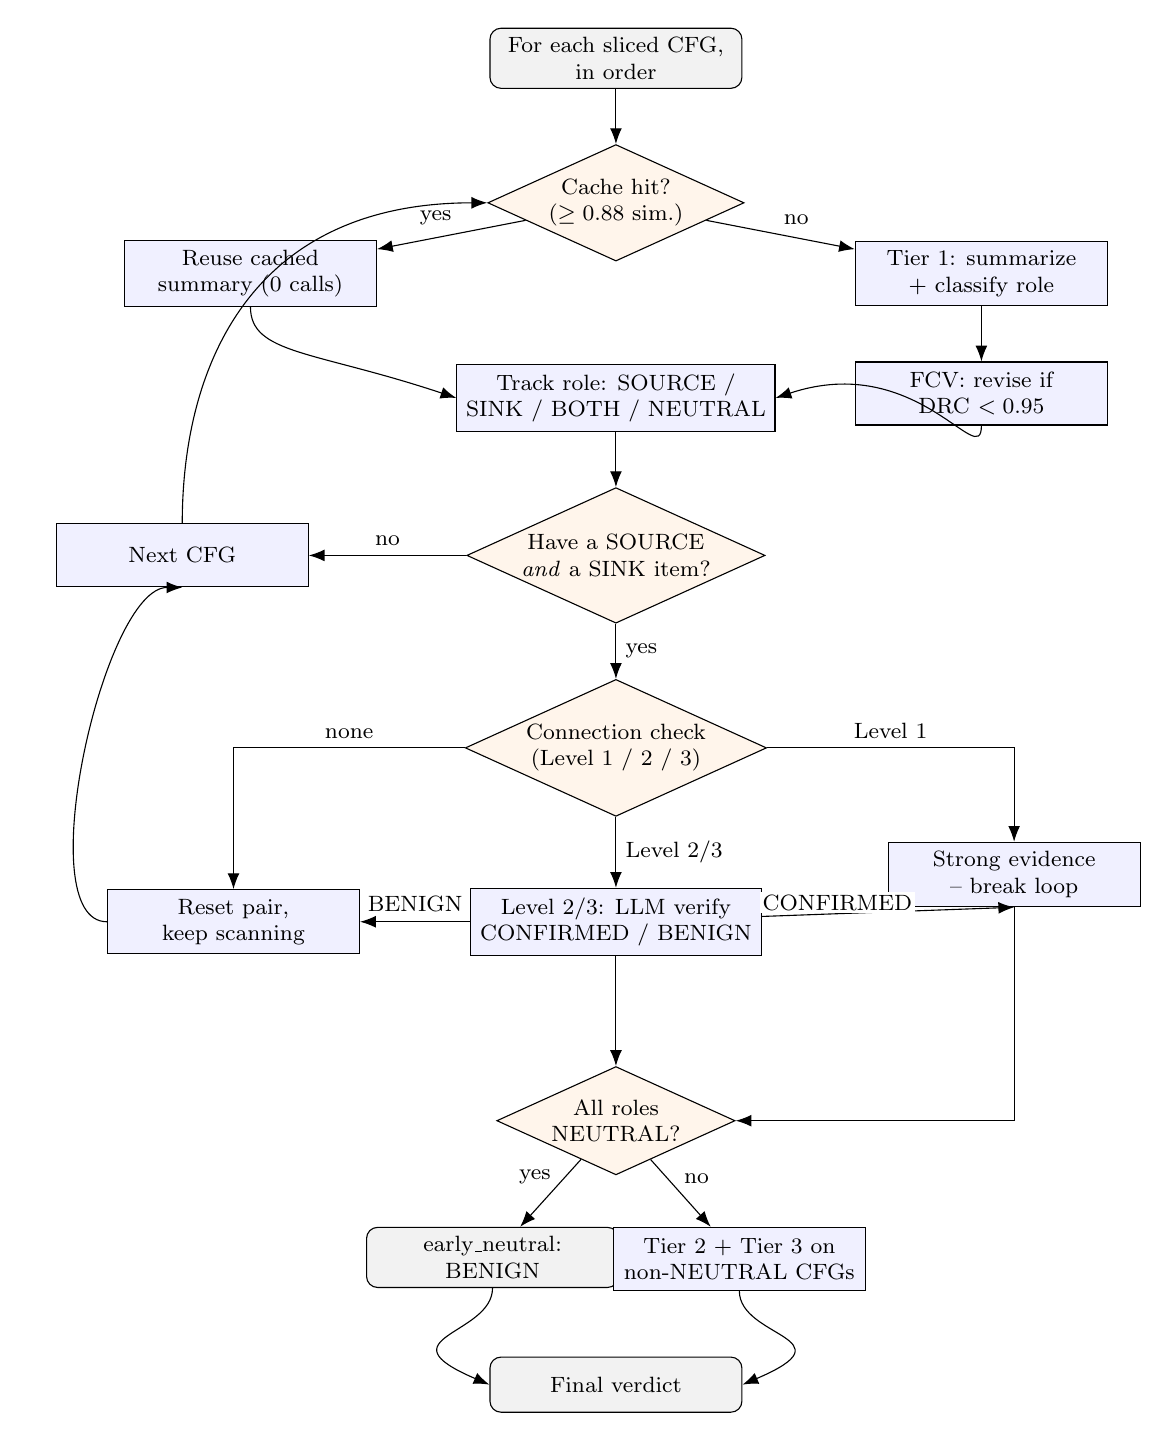
\begin{tikzpicture}[
  node distance=7mm and 10mm,
  every node/.style={font=\footnotesize},
  startstop/.style={rectangle, rounded corners, draw, fill=gray!10, minimum width=32mm, minimum height=7mm, align=center},
  process/.style={rectangle, draw, fill=blue!6, minimum width=32mm, minimum height=8mm, align=center},
  decision/.style={diamond, draw, fill=orange!8, aspect=2.2, inner sep=1pt, align=center},
  arr/.style={-{Latex[length=2mm]}}
]
  \node[startstop] (start) {For each sliced CFG,\\in order};
  \node[decision, below=of start] (cachehit) {Cache hit?\\($\geq 0.88$ sim.)};
  \node[process, left=14mm of cachehit, yshift=-9mm] (reuse) {Reuse cached\\summary (0 calls)};
  \node[process, right=14mm of cachehit, yshift=-9mm] (tier1) {Tier 1: summarize\\+ classify role};
  \node[process, below=of tier1] (fcv) {FCV: revise if\\DRC $< 0.95$};
  \node[process, below=13mm of cachehit] (role) {Track role: SOURCE /\\SINK / BOTH / NEUTRAL};
  \node[decision, below=of role] (pair) {Have a SOURCE\\\emph{and} a SINK item?};
  \node[process, left=20mm of pair] (next) {Next CFG};
  \node[decision, below=of pair] (conn) {Connection check\\(Level 1 / 2 / 3)};
  \node[process, below=9mm of conn] (verify) {Level 2/3: LLM verify\\CONFIRMED / BENIGN};
  \node[process, left=14mm of verify] (reset) {Reset pair,\\keep scanning};
  \node[process, right=16mm of verify, yshift=6mm] (strong) {Strong evidence\\-- break loop};
  \node[decision, below=14mm of verify] (allneutral) {All roles\\NEUTRAL?};
  \node[startstop, below left=10mm and -8mm of allneutral] (benign) {early\_neutral:\\BENIGN};
  \node[process, below right=10mm and -8mm of allneutral] (tier23) {Tier 2 + Tier 3 on\\non-NEUTRAL CFGs};
  \node[startstop, below=9mm of allneutral, yshift=-14mm] (final) {Final verdict};

  \draw[arr] (start) -- (cachehit);
  \draw[arr] (cachehit) -- node[above,xshift=-2mm]{yes} (reuse);
  \draw[arr] (cachehit) -- node[above,xshift=2mm]{no} (tier1);
  \draw[arr] (tier1) -- (fcv);
  \draw[arr] (fcv.south) .. controls +(0,-6mm) and +(18mm,6mm) .. (role.east);
  \draw[arr] (reuse.south) .. controls +(0,-6mm) and +(-18mm,6mm) .. (role.west);
  \draw[arr] (role) -- (pair);
  \draw[arr] (pair) -- node[above]{no} (next);
  \draw[arr] (next.north) .. controls +(0,20mm) and +(-30mm,0) .. (cachehit.west);
  \draw[arr] (pair) -- node[right]{yes} (conn);
  \draw[arr] (conn) -| node[near start, above]{none} (reset.north);
  \draw[arr] (conn) -- node[right]{Level 2/3} (verify);
  \draw[arr] (conn) -| node[near start, above]{Level 1} (strong.north);
  \draw[arr] (verify) -- node[pos=0.3, above, fill=white, inner sep=1pt]{CONFIRMED} (strong.south);
  \draw[arr] (verify) -- node[above]{BENIGN} (reset);
  \draw[arr] (reset.west) .. controls +(-10mm,0) and +(-10mm,0) .. (next.south);
  \draw[arr] (strong.south) |- (allneutral.east);
  \draw[arr] (verify.south) |- ++(0,-8mm) -| (allneutral);
  \draw[arr] (allneutral) -- node[above,xshift=-2mm]{yes} (benign);
  \draw[arr] (allneutral) -- node[above,xshift=2mm]{no} (tier23);
  \draw[arr] (benign.south) .. controls +(0,-6mm) and +(-14mm,6mm) .. (final.west);
  \draw[arr] (tier23.south) .. controls +(0,-6mm) and +(14mm,6mm) .. (final.east);
\end{tikzpicture}
}
\caption{End-to-end flow of the current LAMD-based candidate
(cache-and-verified-connection design). Each sliced CFG either hits the
semantic cache or goes through Tier~1 and FCV; once a SOURCE and a SINK item
have both been seen, a three-level connection check decides whether to treat
them as evidence before the pipeline falls through to Tier~2/3 or an early
verdict.}
\label{fig:lamd-cache-pipeline}
\end{figure}

\section{Datasets}

Development and debugging of the LAMD-based candidate used a small,
purpose-built sample of 12 APKs downloaded live via the AndroZoo API: 7
malware samples (\texttt{vt\_detection} $\geq 15$) and 5 benign samples
(\texttt{vt\_detection} $= 0$, sourced from the Google Play market), each
between 200KB and 1.3MB to keep pipeline runtime tractable during
iteration. This set is a development/debugging sample used to validate and
compare pipeline behavior across design changes (Chapter~\ref{Chapter5}); it
is distinct from the original LAMD paper's own evaluation set, which spans
13,794 AndroZoo samples labeled through VirusTotal ($>4$ engine detections)
across three temporally ordered test periods (2020--2023) to measure
robustness to distribution drift~\cite{Qian2025-ua}. A larger-scale
evaluation dataset for the final cross-candidate comparison has not yet
been finalized. Separately, an unfiltered random sample of 750 AndroZoo
APKs (no confidence threshold, no class balancing) is being run against two
additional self-hosted backends as an in-progress robustness check on the
candidate's false-positive behavior outside the curated 12-APK set; this is
exploratory and distinct from the finalized cross-candidate dataset above --
see Section~\ref{sec:threats-ch5}.

\section{Evaluation Metrics}\label{sec:metrics}

Detection quality is measured with Accuracy, Precision, Recall, and
F1-score, plus False Positive Rate (FPR) and False Negative Rate (FNR) to
separate the two error modes given the class imbalance typical of malware
datasets. Efficiency is measured separately via LLM call count, token usage,
wall-clock runtime per APK, and cost per APK in USD, since LLM-based methods
trade detection quality against non-trivial inference cost
(Chapter~\ref{Chapter3}, RQ2).

\section{Experimental Setup}

\textit{[TODO: Describe prompts/configurations and the procedure used to run
each candidate method once additional candidates are integrated.]}

The LAMD-based candidate is implemented in Python, using androguard for
static analysis and backward slicing, and a persistent semantic cache
(ChromaDB with its default ONNX embedding model) for the CFG-level cache
described in Section~\ref{sec:lamd-candidate}.

\textbf{LLM backend note.} The LAMD paper's own experiments use
GPT-4o-mini~\cite{Qian2025-ua}. For this thesis, all LAMD-based candidate
runs instead use a different backend model, accessed through a CLI-driven
subprocess call rather than a directly billed API, after the originally
planned API-based backend became impractical to sustain during development.
This substitution should be read as a methodology caveat: results produced
in Chapter~\ref{Chapter5} are not directly comparable to the original
paper's published figures on model choice alone. It is, however, consistent
with the original paper's own discussion of API cost as a practical
deployment constraint and its suggestion that cheaper or locally hosted
models are a natural next step.


\chapter{Experimental Results and Discussion}
\label{Chapter5}

\section{Results}

\textit{[TODO: Once additional candidates from Chapter~\ref{Chapter4} are
implemented, report a final cross-candidate comparison table here using the
metrics defined in Section~\ref{sec:metrics}.]}

The results below are an internal ablation of the LAMD-based candidate
only (baseline reimplementation vs.\ its own optimized versions,
Section~\ref{sec:lamd-candidate}), not yet a comparison against other
candidate methods. They were reconstructed from development logs and prior
analysis sessions rather than freshly re-run for this write-up; the exact
figures should be treated as best-available and re-verified before being
cited as final thesis results.

Table~\ref{tab:cache-ablation} isolates the effect of the semantic cache
alone, on a single 24-CFG APK, comparing no cache against a cold cache
(empty at the start of the run) and a warm cache (already populated by a
prior run on similar code). All three configurations agree on the
MALWARE verdict.

Neither configuration was billed per token: the LAMD-based candidate's
backend is accessed through a CLI-driven subprocess under a flat-rate
account rather than a directly billed API (Section~\ref{sec:lamd-candidate}),
so no invoice-level dollar figure exists for these runs. The \emph{estimated}
cost rows below apply the backend model's public list price as of this
writing (\$5 per million input tokens, \$30 per million output tokens) to
the token counts already reported, using the input/output split observed
directly in this candidate's own logged runs ($\approx$70\% input,
$\approx$30\% output) where a per-call split was not separately recorded.
These figures answer "what would this have cost under standard API
billing", not "what was actually paid" -- they are included because
Chapter~\ref{Chapter3}'s RQ2 (Section~\ref{sec:rq2}) treats a per-APK dollar
figure as central to comparing LLM-based detectors, and omitting one
entirely would leave that comparison axis unaddressed for this candidate.

\begin{table}[ht]
\centering
\caption{Effect of the semantic cache on the same 24-CFG APK}
\label{tab:cache-ablation}
\begin{tabular}{@{}lrrr@{}}
\toprule
 & No cache & Cold cache & Warm cache \\
\midrule
LLM calls        & 62      & 30 ($-52\%$)  & \textbf{9 ($-85\%$)} \\
Total tokens      & 146{,}533 & 78{,}749 ($-46\%$) & \textbf{41{,}598 ($-72\%$)} \\
Cache hit rate    & --      & 14/24         & \textbf{24/24} \\
Est.\ cost (USD)$^*$ & \$1.83 & \$0.98 ($-46\%$) & \textbf{\$0.52 ($-72\%$)} \\
Prediction        & MALWARE & MALWARE       & MALWARE \\
\bottomrule
\end{tabular}
\vspace{2pt}
\footnotesize\textit{$^*$Estimated at \$5/1M input + \$30/1M output tokens
(backend list price at time of writing) applied to this run's total token
count via the $\approx$70/30 input/output split observed elsewhere in this
candidate's logs -- not an actual per-token invoice; see text above.}
\end{table}

Table~\ref{tab:paired-comparison} reports a paired baseline-vs-improved
comparison on 6 fresh AndroZoo malware APKs, run once each through the
unoptimized baseline and the current cache-and-verified-connection design.
One case (\texttt{032EF910\ldots}) is excluded from the reduction column: at
the time of this run it exposed the missing-sink-API gap described in
Section~\ref{sec:lamd-candidate}, so the two pipelines used the same evidence
and reached different verdicts by chance rather than by design; after that
fix, the improved pipeline recovers the correct verdict.

\begin{table}[ht]
\centering
\caption{Paired baseline-vs-improved comparison, 6 malware APKs}
\label{tab:paired-comparison}
\begin{tabular}{@{}lrrrl@{}}
\toprule
APK & Baseline calls & Improved calls & Reduction & Prediction \\
\midrule
008C3C11\ldots & 124 & 54 & 56\% & MALWARE (both) \\
019B34A0\ldots & 97  & 48 & 51\% & MALWARE (both) \\
04C5329F\ldots  & 91  & 28 & 69\% & MALWARE (both) \\
05B7569D\ldots  & 89  & 3  & 97\% & MALWARE (both, post-fix) \\
\bottomrule
\end{tabular}
\end{table}

Across the full 12-APK set (7 malware, 5 benign), the improved pipeline
reached the correct verdict on 11/12 samples (91.7\%, rounded to 92\%
elsewhere in this chapter) after both design fixes described in
Section~\ref{sec:lamd-candidate}, up from 10/12 (83\%) before those fixes.
The one remaining miss was traced to Tier-3's verdict not being fully
deterministic across repeated LLM calls on the same borderline evidence,
rather than to either fixed design issue -- noted here as an open point,
discussed further in Section~\ref{sec:threats-ch5}. The miss is itself a
malware sample misclassified as benign (a false negative); the other 6
malware and all 5 benign samples are correct, giving
$\mathrm{TP}=6,\mathrm{FN}=1,\mathrm{TN}=5,\mathrm{FP}=0$, i.e.\ Precision
$=100\%$ and Recall $=85.7\%$ -- the figures quoted in
Section~\ref{sec:threats-ch5}.

\section{Discussion}

\textit{[TODO: Interpret the results. Compare against the related work
reviewed in Chapter~\ref{Chapter2}. Explain any surprising findings, and
directly answer the research questions stated in Chapter~\ref{Chapter1}.]}

\section{Threats to Validity}\label{sec:threats-ch5}

\subsection{Dataset Size and Selection Bias (Primary Threat)}

The 92\% figure above, like every other result in this chapter, is measured
on the 12-APK development set described in Section~\ref{sec:lamd-candidate}:
a small sample hand-curated at extreme VirusTotal confidence
($\texttt{vt\_detection}\geq15$ malware, $\texttt{vt\_detection}=0$ benign)
and balanced 7:5 malware-to-benign. This is the single most consequential
threat to the results in this chapter, and it is not merely a theoretical
concern -- it is directly measurable within this project. A separate,
unfiltered random sample of 750 AndroZoo APKs (no confidence threshold, no
class balancing, i.e.\ a realistic deployment-like distribution) is being
run through the same candidate design on two different self-hosted LLM
backends (``fit'', a locally hosted Qwen3.6-27B, and ``iec'', a second
self-hosted model) -- an in-progress run, 596/750 and 215/750 complete
respectively at time of writing, and the \texttt{fit} figures additionally
mix results from before and after a mid-run dataset rebalance (see caption).
Figure~\ref{fig:dataset-bias} reports accuracy, precision, and recall on
all three.

\begin{figure}[htbp]
\centering
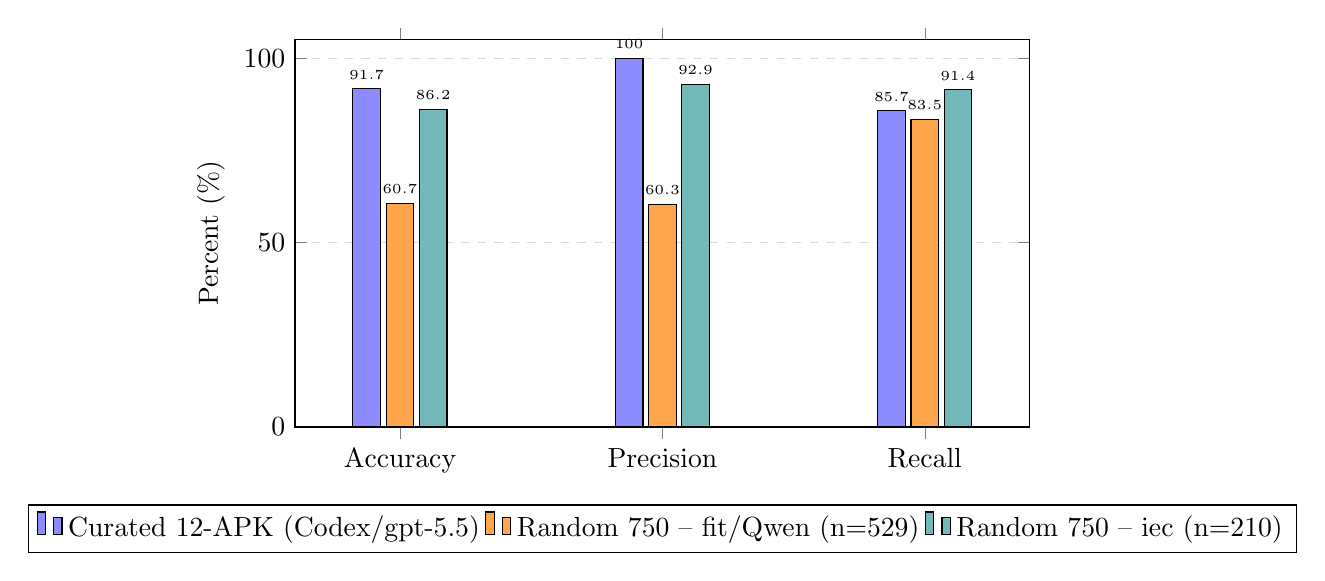
\begin{tikzpicture}
\begin{axis}[
    ybar,
    bar width=10pt,
    width=0.9\textwidth,
    height=6.5cm,
    ymin=0, ymax=105,
    ylabel={Percent (\%)},
    symbolic x coords={Accuracy, Precision, Recall},
    xtick=data,
    enlarge x limits=0.2,
    legend style={at={(0.5,-0.2)}, anchor=north, legend columns=-1},
    nodes near coords,
    nodes near coords align={vertical},
    every node near coord/.append style={font=\tiny},
    ymajorgrids=true,
    grid style={dashed, gray!30},
]
\addplot[fill=blue!45] coordinates {(Accuracy,91.7) (Precision,100) (Recall,85.7)};
\addplot[fill=orange!70] coordinates {(Accuracy,60.7) (Precision,60.3) (Recall,83.5)};
\addplot[fill=teal!55] coordinates {(Accuracy,86.2) (Precision,92.9) (Recall,91.4)};
\legend{Curated 12-APK (Codex/gpt-5.5), Random 750 -- fit/Qwen (n=529), Random 750 -- iec (n=210)}
\end{axis}
\end{tikzpicture}
\caption{Detection performance on the curated 12-APK development set versus
an in-progress, unfiltered random sample of 750 AndroZoo APKs run on two
different backends. Figures for the random sample reflect partial progress
at the time of writing (596/750 fit, 215/750 iec) and will change as the
run completes; the \texttt{fit} column additionally mixes results from
before and after a mid-run dataset rebalance (25\% of the 750 pool was
swapped to reach a 50:50 malware:benign split partway through), so it
should be read as directional, not final. Recomputed via
\texttt{results/compute\_accuracy.py} against ground truth reconstructed
from the original AndroZoo VirusTotal metadata.}
\label{fig:dataset-bias}
\end{figure}

Recall holds up across all three (83.5--91.4\%), so the pipeline is not
missing more real malware on the unfiltered sample. Precision, however,
diverges sharply by \emph{backend}: on \texttt{iec} it stays close to the
curated set (92.9\% vs.\ 100\%), while on \texttt{fit} it collapses to
60.3\%. Since the curated 12-APK figures were themselves produced on a
third backend (Codex CLI/gpt-5.5, Section~\ref{sec:lamd-candidate}), this
comparison cannot cleanly separate a ``dataset difficulty'' effect from a
``backend'' effect -- both vary at once between the curated and random
runs, and the \texttt{fit} vs.\ \texttt{iec} gap on the \emph{same}
unfiltered sample shows the backend effect alone is already large. What
can be said without that confound: the pipeline's false-positive behavior
is not a fixed property of the design, and evaluating it on one
easy, class-balanced, high-confidence, single-backend sample --
as the 92\% headline figure in this chapter does -- is not sufficient to
characterize it. Root-caused false positives on the \texttt{fit} run trace
to legitimate-but-suspicious-looking patterns (e.g.\ login flows that read
credential fields before a network call, or reflection-based library
internals such as OkHttp's certificate-chain cleaner) that the curated
set's hand-picked samples do not happen to exercise. The 92\% headline
figure should therefore be read as an upper-bound, best-case result under
favorable sampling \emph{and} backend conditions, not as a general-purpose
accuracy estimate; Chapter~\ref{Chapter6} returns to this point when
scoping the thesis's claims.

\subsection{Other Threats}

\textbf{LLM non-determinism.} As noted above, the one remaining miss on
the 12-APK set was traced to Tier~3
producing different verdicts across repeated calls on byte-identical
upstream evidence -- inherent sampling variance in the backend model
rather than a pipeline defect. This means the reported accuracy figures
are themselves a single draw from a distribution rather than a fully
reproducible number; a self-consistency or majority-vote Tier~3 (calling
the final verdict step multiple times and taking the majority) was
discussed as a candidate mitigation but not implemented, since it would
proportionally increase the per-APK cost figures reported in
Section~\ref{sec:metrics}.

\textbf{Cache similarity threshold.} The semantic cache's reuse threshold
(cosine similarity $\geq0.88$, Section~\ref{sec:lamd-candidate}) was fixed
by inspection rather than swept experimentally. No sensitivity analysis
was run to check how cache-hit rate, cost, or downstream accuracy would
change at a stricter or looser threshold, so the reported cost savings in
Section~\ref{sec:metrics} should be read as specific to this one setting,
not necessarily its optimum.


\chapter{Conclusion and Future Work}
\label{Chapter6}

\section{Summary}

This thesis set out to evaluate LLM-based Android malware detection under a
common framework, treating detection quality and cost-efficiency as
co-equal evaluation axes rather than reporting cost as an afterthought to
accuracy (Chapter~\ref{Chapter4}). The first phase was a Systematic
Literature Review of six primary studies (Chapter~\ref{Chapter3}), which
mapped the field into three recurring strategies (Retrieval-Augmented
Generation, Semantic Representation, and Fine-tuning/Direct
Classification), synthesized their reported effectiveness and cost
profiles without over-claiming direct numerical comparability, and
identified concrete gaps: inconsistent cost reporting, a shared reliance
on static analysis alone, and reliability limits from hallucination and
prompt sensitivity. The second phase built and iteratively hardened one
concrete candidate on top of the LAMD framework (Chapter~\ref{Chapter4}),
progressing from a faithful baseline reimplementation through role-based
early exit, a semantic cache, and multi-level SOURCE/SINK connection
verification, with each optimization's own accuracy risk found and fixed
before being accepted (Table~\ref{tab:design-history}). The measured
results (Chapter~\ref{Chapter5}) show the two cost-reduction mechanisms
working as designed -- up to 85\% fewer LLM calls and 72\% fewer tokens
from the cache alone, 51--97\% fewer calls from connection-verified early
exit -- without changing the verdict on the cases tested, and 11/12 (92\%)
correct on the curated development set. The same results also show this
headline figure does not generalize on its own: on an unfiltered random
sample, precision held near the curated figure on one backend (92.9\%,
\texttt{iec}) but collapsed on another (60.3\%, \texttt{fit}/Qwen), showing
that the accuracy story is backend-dependent as much as it is
dataset-dependent.

\section{Contributions and Significance}

This thesis's contributions are scoped honestly to what was actually built,
not to the fuller cross-candidate comparison originally targeted
(Chapter~\ref{Chapter4}). As of this writing, one
candidate has a working, measured implementation; the significance below
follows from that one candidate, not from a comparison across methods.

\textbf{A measured, not asserted, cost-efficiency result.} The literature
surveyed in Chapter~\ref{Chapter3} identifies cost as a persistent, poorly
standardized concern across LLM-based detectors (RQ2, RQ3) but rarely
isolates which specific design choice buys which specific saving. This
thesis contributes a design history (Table~\ref{tab:design-history}) that
attributes each cost reduction to a specific, independently-tested
mechanism -- caching versus connection-verified early exit -- with paired
before/after numbers for each, rather than a single aggregate saving
figure whose source is hard to attribute.

\textbf{Evidence that cost-saving and correctness-preserving are separate
engineering problems.} The same design history shows, with dated,
root-caused examples, that a cost-reduction mechanism which appears to
work (naive early exit; same-class connection without verification) can
silently change a verdict, and that closing each gap was a distinct
engineering step, not a byproduct of the original optimization. This is a
concrete, reproducible instance of a pattern the surveyed literature
discusses more abstractly (Chapter~\ref{Chapter3}, RQ3's discussion of
verification mechanisms being themselves susceptible to error).

\textbf{Empirical confirmation, on a fresh sample, of two gaps the SLR
identified from the literature alone.} The unfiltered 750-APK comparison
(Section~\ref{sec:threats-ch5}) is independent evidence -- not a citation
of prior work -- for two claims Chapter~\ref{Chapter3} makes from reading
other papers: that reliance on static analysis alone leaves a persistent
blind spot (confirmed here by a real missed detection carried entirely in
a native \texttt{.so} library, Chapter~\ref{Chapter5}), and that
verification mechanisms do not catch every reliability failure (confirmed
here by false positives that are structurally accurate but semantically
misjudged, evading LAMD's own Factual Consistency Verification).

\textbf{A reusable evaluation framework.} Independent of any single
candidate's results, Chapter~\ref{Chapter4}'s dataset, metric, and
protocol definitions are built to accept additional candidates from the
Chapter~\ref{Chapter3} taxonomy without redefinition, which is the
practical prerequisite for the cross-candidate comparison this thesis did
not have time to complete.

\section{Limitations}\label{sec:limitations-ch6}

The measurement-level limitations of the results already reported --
sample size, LLM non-determinism, an unswept cache threshold -- are
discussed in Section~\ref{sec:threats-ch5} and are not repeated here. This
section instead states the boundaries of what the thesis attempted at
all.

\textbf{Scope: one candidate, not a comparison.} The thesis's own stated
goal (Chapter~\ref{Chapter4}) was a common framework for comparing
multiple LLM-based candidates. Only one candidate reached a working,
measured implementation. Every accuracy, cost, and reliability finding in
this thesis is therefore a finding about the LAMD-based design
specifically, not a general claim about LLM-based Android malware
detection as a class.

\textbf{The 750-APK evaluation is unfinished.} The random-sample
comparison central to Chapter~\ref{Chapter5}'s Discussion and Threats to
Validity was, at the time of writing, an in-progress run (596/750 and
215/750 complete on the two backends), and the \texttt{fit} backend's
figures mix pre- and post-rebalance results from a dataset composition
change made partway through. The directional finding -- precision is
backend-dependent -- is unlikely to reverse, but the exact percentages
reported are not final numbers.

\textbf{The RAG-grounding exploration is not a second candidate.} A
retrieval-augmented prompt-grounding technique was implemented and tested
on top of the LAMD-based candidate (Chapter~\ref{Chapter4}), but it was
never evaluated under the common framework's accuracy/cost metrics on more
than a single APK, and it reuses the LAMD-based candidate's own pipeline
rather than constituting an independent detection architecture. It is
reported as an internal exploration, not as evidence toward a second,
independently-evaluated candidate.

\section{Future Work}

\textbf{Complete the in-progress 750-APK evaluation.} The clearest
near-term action is finishing the random-sample run on both backends and
recomputing Section~\ref{sec:threats-ch5}'s figures on the full,
post-rebalance 750 APKs, since the current numbers are explicitly
provisional.

\textbf{Address Tier-3 non-determinism.} A self-consistency or
majority-vote Tier-3 (issuing the final-verdict call multiple times and
taking the majority) was discussed as a candidate fix during development
(Section~\ref{sec:threats-ch5}) but not implemented, since it
proportionally increases per-APK cost -- itself a concrete instance of the
cost/reliability trade-off this thesis's cost-efficiency framing puts
front and center, and a natural next design-history entry to measure
rather than assume.

\textbf{Sweep the cache similarity threshold.} The $\geq 0.88$ cosine
threshold was fixed by inspection; a systematic sweep would show whether
cache-hit rate, cost, and downstream accuracy trade off favorably at other
settings, closing the gap noted in Section~\ref{sec:threats-ch5}.

\textbf{Implement additional candidates to complete the cross-candidate
comparison.} This is the most direct way to close the scope gap in
Section~\ref{sec:limitations-ch6} above: at least one RAG-based and one
fine-tuning-based candidate, representative of the two families identified
in Chapter~\ref{Chapter3}'s taxonomy (RQ1) but not yet implemented here,
would let Chapter~\ref{Chapter4}'s evaluation framework fulfill its
original purpose.

\textbf{Evaluate a cascaded triage architecture.} Chapter~\ref{Chapter5}'s
Discussion motivates this concretely, not abstractly: the false-positive
pattern observed on the \texttt{fit} backend (ordinary login flows,
common bundled-library reflection patterns) is the kind of case a
lightweight pre-filter could plausibly screen out before full LLM
reasoning is invoked, in the spirit of Chapter~\ref{Chapter3}'s RQ4
recommendation, and this thesis's own false-positive data is a ready-made
test set for that idea.


% Author's publications (comment out the two lines below if there are none)
\addcontentsline{toc}{chapter}{List of Publications}
\chapter*{List of Publications}
\label{publications}

\begin{enumerate}
\item \textit{[Systematic literature review on LLM-based Android malware
detection -- add full citation once submitted/accepted.]}
\end{enumerate}


% References
\addcontentsline{toc}{chapter}{References}
\printbibheading[title={References}]

\printbibliography[heading=subbibliography, title={Vietnamese}, keyword=Viet, resetnumbers=true]

\DeclareNameAlias{sortname}{last-first}
\DeclareNameAlias{default}{last-first}

\printbibliography[heading=subbibliography, title={English}, notkeyword=Viet, resetnumbers=4]
% ===================================================================== %
% NOTE: set resetnumbers = (number of Vietnamese references) + 1        %
% ===================================================================== %

% Appendices
\appendix

\chapter{Additional Experimental Data}
\label{Appendix1}

\textit{[Include supplementary data that supports Chapter~\ref{Chapter4} but
is too long for the main text, e.g. full per-sample results, extended
configuration tables, or additional plots.]}

\chapter{LaTeX Formatting Reference}
\label{Appendix2}

This appendix collects short, working examples of the LaTeX constructs most
commonly needed while writing the thesis. It is not part of the thesis
narrative -- it is a quick reference for the authors while editing.

\section{Citations}

Use \verb|\cite| to cite one or more references. A reference can be a
website~\cite{Listings,HDLVThS}, a conference paper~\cite{1994-Cavnar}, a
book~\cite{1984-TeX-Knuth,2006-DDien,2006-NPTV}, or a journal
article~\cite{1989-TED}. Write sentences so that they still read correctly
if the bracketed citation were removed -- prefer ``Zhang and
Shasha~\cite{1989-TED} show that ...'' over ``Research~\cite{1989-TED} shows
that ...''.

\section{Source Code}

Source code listings use the \verb|listings| package~\cite{Listings}. Code
can be inserted inline:

\begin{lstlisting}[language=Python]
print("Hello, World!")
\end{lstlisting}

or included from a file in \verb|SourceCode/|:

\lstinputlisting[language=C++]{SourceCode/hello.cpp}

Pseudocode uses the \verb|algorithm|/\verb|algpseudocode| packages:

\begin{algorithm}
\caption{Example algorithm}\label{euclid}
\begin{algorithmic}[1]
\Procedure{MyProcedure}{}
\State $\textit{stringlen} \gets \text{length of }\textit{string}$
\State $i \gets \textit{patlen}$
\BState \emph{top}:
\If {$i > \textit{stringlen}$} \Return false
\EndIf
\State $j \gets \textit{patlen}$
\BState \emph{loop}:
\If {$\textit{string}(i) = \textit{path}(j)$}
\State $j \gets j-1$.
\State $i \gets i-1$.
\State \textbf{goto} \emph{loop}.
\State \textbf{close};
\EndIf
\State $i \gets i+\max(\textit{delta}_1(\textit{string}(i)),\textit{delta}_2(j))$.
\State \textbf{goto} \emph{top}.
\EndProcedure
\end{algorithmic}
\end{algorithm}

\section{Figures}

Figures use the \verb|graphicx| package~\cite{Figures}. Figures
\ref{fig:example1} and \ref{fig:example2} show examples.

\begin{figure}[htp]
\centering

\includegraphics[width=9cm]{images/logo.png}
\caption{Example figure 1}
\label{fig:example1}
\end{figure}

\begin{figure*}[htp]
\centering

\includegraphics[width=60mm]{images/logo.png}
\caption{Example figure 2}
\label{fig:example2}
\end{figure*}

\section{Tables}

See~\cite{Tables} for more table examples. Table~\ref{tab:example1} shows a
sample table; \url{http://www.tablesgenerator.com/} can help build tables
visually.

\begin{table}[ht]
\caption{Example table}
\label{tab:example1}
\begin{center}
\begin{tabular}{ |p{3cm}||p{3cm}|p{3cm}|p{3cm}|  }
 \hline
 \multicolumn{4}{|c|}{Country List} \\
 \hline
 Country/Area Name & ISO ALPHA 2 & ISO ALPHA 3 & ISO Numeric \\
 \hline
 Afghanistan   & AF  & AFG & 004\\
 Aland Islands & AX  & ALA & 248\\
 Albania       & AL  & ALB & 008\\
 Algeria       & DZ  & DZA & 012\\
 \hline
\end{tabular}
\end{center}
\end{table}

\section{Equations}

An equation can appear inline, e.g. $\sqrt{a^2+b^2}$, or on its own line as
in Equation~\ref{eu_eqn}.

\begin{equation} \label{eu_eqn}
x = a_0 + \frac{1}{a_1 + \frac{1}{a_2 + \frac{1}{a_3 + a_4}}}
\end{equation}

\section{General Formatting Rules (FIT/HCMUS)}

\begin{itemize}
\item Font: Times New Roman (Unicode), 13-14pt; 1.5 line spacing.
\item Margins: top 3cm, bottom 3.5cm, left 3.5cm, right 2cm; page number
centered at the bottom.
\item Length: 50-100 pages of content (excluding cover, acknowledgments,
table of contents, references, appendices).
\item Number chapters/sections/subsections with Arabic numerals only
(e.g.\ \texttt{3.1}, \texttt{3.1.1}), never Roman numerals.
\item Figure/table/equation numbers are tied to the chapter number, e.g.\
Figure 3.4 is the 4th figure in Chapter 3. Always cite the source of any
figure/table taken from elsewhere.
\item Avoid overusing abbreviations; list them alphabetically at the front of
the thesis if there are many.
\end{itemize}


\end{document}
